\documentclass[journal]{IEEEtran}
%DIF LATEXDIFF DIFFERENCE FILE
%DIF DEL old/main.tex   Tue Oct 20 10:58:46 2026
%DIF ADD new/main.tex   Tue Oct 20 10:58:45 2026

\usepackage{cite}
\usepackage{xspace}

% to be able to draw some self-contained figs
\usepackage{tikz}
\usepackage{graphicx}
\usepackage{amsmath}

% my coustom packages
\usepackage{paralist}
\usepackage{enumitem}
\usepackage{amssymb}
\usepackage{booktabs}
\usepackage{tabularx}
\usepackage{pifont}
\usepackage{environ}
\usepackage{subcaption}

\usepackage{fvextra}
\usepackage{fancyvrb}
\usepackage{url}
\usepackage{hyperref}
% \usepackage{titling}

% --------- DEFINE COLORS ---------
% Blue 系
\definecolor{xblue}{RGB}{76,114,176}        % 沉稳学术蓝
\definecolor{navy}{RGB}{59,72,99}           % 深藏青
\definecolor{steelblue}{RGB}{102,139,171}   % 钢蓝

% Red 系
\definecolor{xred}{RGB}{172,31,24}           % 暗红（非警告型）
\definecolor{maroon}{RGB}{128,70,70}        % 学术酒红
\definecolor{brick}{RGB}{150,90,75}         % 砖红

% Green 系
\definecolor{xgreen}{RGB}{90,140,120}        % 灰绿色
\definecolor{olive}{RGB}{120,130,90}        % 橄榄绿
\definecolor{forest}{RGB}{80,110,95}        % 深林绿

% Yellow / Orange 系
\definecolor{xorange}{RGB}{200,140,90}       % 低饱和橙
\definecolor{goldenrod}{RGB}{170,145,85}    % 学术金
\definecolor{sand}{RGB}{190,175,140}        % 沙色

% Purple 系
\definecolor{xpurple}{RGB}{130,110,150}      % 灰紫
\definecolor{plum}{RGB}{120,95,125}         % 李子紫
\definecolor{violet}{RGB}{145,130,170}      % 冷紫

% Gray 系（强烈推荐学术使用）
\definecolor{xgray}{RGB}{130,130,130}
\definecolor{darkgray}{RGB}{90,90,90}
\definecolor{lightgray}{RGB}{200,200,200}
% ---------------------------------

% my coustom commands
\newcommand{\rom}[1]{\romannumeral #1}
\newcommand{\Rom}[1]{\uppercase\expandafter{\romannumeral #1}}


\newcommand{\funcText}[1]{{\ttfamily #1}}

\newcommand{\ruleNameText}[1]{{\ttfamily #1}}

\newcommand{\TFact}[1]{{\ttfamily #1}}
\newcommand{\TLemma}[1]{{\ttfamily #1}}
\newcommand{\TEmpFact}[1]{\lbrack \  #1 \rbrack}
\newcommand{\TFacts}[1]{\lbrack\ #1 \ \rbrack}
\newcommand{\TEmpActFact}[0]{-\hspace{-0.45em}\rightarrow}
\newcommand{\TEmpActFactSL}[1]{- \hspace{-3.6pt} \TEmpFact{#1} \hspace{-4.2pt} \rightarrow} % single line
\newcommand{\TActFacts}[1]{- \hspace{-4.5pt} \TFacts{#1} \hspace{-4.8pt} \rightarrow}
\newcommand{\TActFactsSL}[1]{- \hspace{-3.7pt} \TFacts{#1} \hspace{-4.2pt} \rightarrow}
\newcommand{\TPair}[1]{\langle #1 \rangle}
\newcommand{\TPairN}[1]{$\langle$\text{\ttfamily #1}$\rangle$}

\newcommand{\TLet}[0]{\text{\Tterm{let}}}
\newcommand{\TIn}[0]{\text{\Tterm{in}}}

\newcommand{\TLetS}[0]{\text{\Tterm{let}} \hspace{0.5em}}
\newcommand{\TInS}[0]{\text{\Tterm{in}} \hspace{0.5em}}

\newcommand{\TAll}[0]{\text{\textcolor{xred}{\TLemma{All}}}}
\newcommand{\TEx}[0]{\text{\textcolor{xgreen!80!black}{\TLemma{Ex}}}}
\newcommand{\TNot}[0]{\text{\TLemma{not}}}

\newcommand{\Tterm}[1]{{\ttfamily #1}}
\newcommand{\Tequation}[1]{{\ttfamily #1}}
\newcommand{\Tfunction}[1]{{\ttfamily #1}}
\newcommand{\Tamarin}{Tamarin-Prover\xspace}

\newcommand{\TFrTerm}[1]{{\Tterm{$\sim$#1}}}
\newcommand{\TFactTerm}[2]{{\ttfamily #1}$(\,$\Tterm{#2}$\,)$}
\newcommand{\TFrFactTerm}[1]{{\ttfamily Fr}$(\,$\TFrTerm{#1}$\,)$}

\newcommand{\TSymbolFr}[0]{\text{\textasciitilde}}

% \setlist[enumerate]{
%   itemsep=0pt,
%   topsep=2pt
% }

\NewEnviron{tightflalign}{%
  {%
    \setlength{\abovedisplayskip}{6pt}%
    \setlength{\belowdisplayskip}{6pt}%
    \begin{flalign*}
      \BODY
    \end{flalign*}
  }%
}



\usepackage{soul}
\soulregister\cite7
\soulregister\ref7
\soulregister\eqref7
\soulregister\Rom7
\soulregister\ding7
\newcommand{\modify}[1]{#1}
% \newcommand{\modify}[1]{\textcolor{blue!30!xblue}{\ul{#1}}}
\newcommand{\outline}[1]{#1}
% \newcommand{\outline}[1]{\textcolor{red!30!xred}{\ul{#1}}}

%-------------------------------------------------------------------------------
%DIF PREAMBLE EXTENSION ADDED BY LATEXDIFF
%DIF UNDERLINE PREAMBLE %DIF PREAMBLE
\RequirePackage[normalem]{ulem} %DIF PREAMBLE
\RequirePackage{color}\definecolor{RED}{rgb}{1,0,0}\definecolor{BLUE}{rgb}{0,0,1} %DIF PREAMBLE
\providecommand{\DIFaddtex}[1]{{\protect\color{blue}\uwave{#1}}} %DIF PREAMBLE
\providecommand{\DIFdeltex}[1]{{\protect\color{red}\sout{#1}}} %DIF PREAMBLE
%DIF SAFE PREAMBLE %DIF PREAMBLE
\providecommand{\DIFaddbegin}{} %DIF PREAMBLE
\providecommand{\DIFaddend}{} %DIF PREAMBLE
\providecommand{\DIFdelbegin}{} %DIF PREAMBLE
\providecommand{\DIFdelend}{} %DIF PREAMBLE
\providecommand{\DIFmodbegin}{} %DIF PREAMBLE
\providecommand{\DIFmodend}{} %DIF PREAMBLE
%DIF FLOATSAFE PREAMBLE %DIF PREAMBLE
\providecommand{\DIFaddFL}[1]{\DIFadd{#1}} %DIF PREAMBLE
\providecommand{\DIFdelFL}[1]{\DIFdel{#1}} %DIF PREAMBLE
\providecommand{\DIFaddbeginFL}{} %DIF PREAMBLE
\providecommand{\DIFaddendFL}{} %DIF PREAMBLE
\providecommand{\DIFdelbeginFL}{} %DIF PREAMBLE
\providecommand{\DIFdelendFL}{} %DIF PREAMBLE
%DIF HYPERREF PREAMBLE %DIF PREAMBLE
\providecommand{\DIFadd}[1]{\texorpdfstring{\DIFaddtex{#1}}{#1}} %DIF PREAMBLE
\providecommand{\DIFdel}[1]{\texorpdfstring{\DIFdeltex{#1}}{}} %DIF PREAMBLE
\providecommand{\DIFscaledelfig}{0.5}
%DIF HIGHLIGHTGRAPHICS PREAMBLE %DIF PREAMBLE
\RequirePackage{settobox} %DIF PREAMBLE
\RequirePackage{letltxmacro} %DIF PREAMBLE
\newsavebox{\DIFdelgraphicsbox} %DIF PREAMBLE
\newlength{\DIFdelgraphicswidth} %DIF PREAMBLE
\newlength{\DIFdelgraphicsheight} %DIF PREAMBLE
% store original definition of \includegraphics %DIF PREAMBLE
\LetLtxMacro{\DIFOincludegraphics}{\includegraphics} %DIF PREAMBLE
\providecommand{\DIFaddincludegraphics}[2][]{{\color{blue}\fbox{\DIFOincludegraphics[#1]{#2}}}} %DIF PREAMBLE
\providecommand{\DIFdelincludegraphics}[2][]{% %DIF PREAMBLE
\sbox{\DIFdelgraphicsbox}{\DIFOincludegraphics[#1]{#2}}% %DIF PREAMBLE
\settoboxwidth{\DIFdelgraphicswidth}{\DIFdelgraphicsbox} %DIF PREAMBLE
\settoboxtotalheight{\DIFdelgraphicsheight}{\DIFdelgraphicsbox} %DIF PREAMBLE
\scalebox{\DIFscaledelfig}{% %DIF PREAMBLE
\parbox[b]{\DIFdelgraphicswidth}{\usebox{\DIFdelgraphicsbox}\\[-\baselineskip] \rule{\DIFdelgraphicswidth}{0em}}\llap{\resizebox{\DIFdelgraphicswidth}{\DIFdelgraphicsheight}{% %DIF PREAMBLE
\setlength{\unitlength}{\DIFdelgraphicswidth}% %DIF PREAMBLE
\begin{picture}(1,1)% %DIF PREAMBLE
\thicklines\linethickness{2pt} %DIF PREAMBLE
{\color[rgb]{1,0,0}\put(0,0){\framebox(1,1){}}}% %DIF PREAMBLE
{\color[rgb]{1,0,0}\put(0,0){\line( 1,1){1}}}% %DIF PREAMBLE
{\color[rgb]{1,0,0}\put(0,1){\line(1,-1){1}}}% %DIF PREAMBLE
\end{picture}% %DIF PREAMBLE
}\hspace*{3pt}}} %DIF PREAMBLE
} %DIF PREAMBLE
\LetLtxMacro{\DIFOaddbegin}{\DIFaddbegin} %DIF PREAMBLE
\LetLtxMacro{\DIFOaddend}{\DIFaddend} %DIF PREAMBLE
\LetLtxMacro{\DIFOdelbegin}{\DIFdelbegin} %DIF PREAMBLE
\LetLtxMacro{\DIFOdelend}{\DIFdelend} %DIF PREAMBLE
\DeclareRobustCommand{\DIFaddbegin}{\DIFOaddbegin \let\includegraphics\DIFaddincludegraphics} %DIF PREAMBLE
\DeclareRobustCommand{\DIFaddend}{\DIFOaddend \let\includegraphics\DIFOincludegraphics} %DIF PREAMBLE
\DeclareRobustCommand{\DIFdelbegin}{\DIFOdelbegin \let\includegraphics\DIFdelincludegraphics} %DIF PREAMBLE
\DeclareRobustCommand{\DIFdelend}{\DIFOaddend \let\includegraphics\DIFOincludegraphics} %DIF PREAMBLE
\LetLtxMacro{\DIFOaddbeginFL}{\DIFaddbeginFL} %DIF PREAMBLE
\LetLtxMacro{\DIFOaddendFL}{\DIFaddendFL} %DIF PREAMBLE
\LetLtxMacro{\DIFOdelbeginFL}{\DIFdelbeginFL} %DIF PREAMBLE
\LetLtxMacro{\DIFOdelendFL}{\DIFdelendFL} %DIF PREAMBLE
\DeclareRobustCommand{\DIFaddbeginFL}{\DIFOaddbeginFL \let\includegraphics\DIFaddincludegraphics} %DIF PREAMBLE
\DeclareRobustCommand{\DIFaddendFL}{\DIFOaddendFL \let\includegraphics\DIFOincludegraphics} %DIF PREAMBLE
\DeclareRobustCommand{\DIFdelbeginFL}{\DIFOdelbeginFL \let\includegraphics\DIFdelincludegraphics} %DIF PREAMBLE
\DeclareRobustCommand{\DIFdelendFL}{\DIFOaddendFL \let\includegraphics\DIFOincludegraphics} %DIF PREAMBLE
%DIF AMSMATHULEM PREAMBLE %DIF PREAMBLE
\makeatletter %DIF PREAMBLE
\let\sout@orig\sout %DIF PREAMBLE
\renewcommand{\sout}[1]{\ifmmode\text{\sout@orig{\ensuremath{#1}}}\else\sout@orig{#1}\fi} %DIF PREAMBLE
\makeatother %DIF PREAMBLE
%DIF COLORLISTINGS PREAMBLE %DIF PREAMBLE
\RequirePackage{listings} %DIF PREAMBLE
\RequirePackage{color} %DIF PREAMBLE
\lstdefinelanguage{DIFcode}{ %DIF PREAMBLE
%DIF DIFCODE_UNDERLINE %DIF PREAMBLE
  moredelim=[il][\color{red}\sout]{\%DIF\ <\ }, %DIF PREAMBLE
  moredelim=[il][\color{blue}\uwave]{\%DIF\ >\ } %DIF PREAMBLE
} %DIF PREAMBLE
\lstdefinestyle{DIFverbatimstyle}{ %DIF PREAMBLE
	language=DIFcode, %DIF PREAMBLE
	basicstyle=\ttfamily, %DIF PREAMBLE
	columns=fullflexible, %DIF PREAMBLE
	keepspaces=true %DIF PREAMBLE
} %DIF PREAMBLE
\lstnewenvironment{DIFverbatim}[1][]{\lstset{style=DIFverbatimstyle}}{} %DIF PREAMBLE
\lstnewenvironment{DIFverbatim*}[1][]{\lstset{style=DIFverbatimstyle,showspaces=true}}{} %DIF PREAMBLE
\lstset{extendedchars=\true,inputencoding=utf8}

%DIF END PREAMBLE EXTENSION ADDED BY LATEXDIFF

\begin{document}
%-------------------------------------------------------------------------------

\title{Formal Analysis and Fixing of Third-Party Online Payment Protocols}

\author{Yongkang~Xiao,
        Jing~Chen,~\IEEEmembership{Senior~Member,~IEEE,}
        Min~Shi,
        Kun~He,~\IEEEmembership{Member,~IEEE,}
        Qiyi~Deng,
        and~Ruiying~Du%
\thanks{Y. Xiao, J. Chen, M. Shi, K. He, Q. Deng, and R. Du are with the School of Cyber Science and Engineering, Wuhan University, Wuhan, China (e-mail: \{xiaoyongkang, chenjing, itachi, hekun, qiyideng, duraying\}@whu.edu.cn). (Corresponding authors: Jing Chen and Min Shi.)}%
\thanks{A preliminary version of this paper appears in the Proceedings of the 35th USENIX Security Symposium (USENIX Security '26)~\cite{xiao2026authorization}. This version presents a new countermeasure, Sealed Checkout Code, together with its formal verification.}}

\markboth{IEEE Transactions on Dependable and Secure Computing}%
{Xiao \MakeLowercase{\textit{et al.}}: Formal Analysis and Fixing of Third-Party Online Payment Protocols}

\maketitle

%-------------------------------------------------------------------------------
\begin{abstract}
%-------------------------------------------------------------------------------
Third-party online payment systems, such as Alipay and PSP-B, constitute critical infrastructure for modern e-commerce.
However, their security rests on the unrealistic assumption of fully trusted communication channels. 
While prior studies have identified isolated vulnerabilities, a systematic formal analysis of payment protocol security remains absent. 
\DIFdelbegin \DIFdel{This paper presents formal security models for }\DIFdelend \DIFaddbegin \DIFadd{We formally model }\DIFaddend six third-party payment protocols, spanning three major payment scenarios and two dominant payment service providers. 
Our analysis reveals a fundamental design flaw: 
whenever channel integrity is compromised between the merchant client, merchant server, or payment system, order tampering attacks become feasible.
We validate this threat on Android, where over \DIFdelbegin \DIFdel{20}\DIFdelend \DIFaddbegin \DIFadd{25}\DIFaddend \% of tested merchant applications allow order tampering through implicit Intent hijacking.
\DIFdelbegin \DIFdel{To mitigate this threat, we propose user-side order authentication, where per-user-merchant key pairs cryptographically bind consent to order semantics.
Formal verification demonstrates its resilience against identified attacks under weak channel assumptions}\DIFdelend \DIFaddbegin \DIFadd{We propose Sealed Checkout Code (SCC): the merchant frontend seals a fresh nonce to the payment system together with the order handle and the user's account, and the user confirms the payment by entering a short code derived from that nonce.
SCC protects every payment without per-user keys or trust on first use, and formal verification shows that it satisfies all security properties when both external channels are insecure}\DIFaddend .
By bridging formal methods and empirical analysis, this work offers actionable guidance for standardizing secure payment protocols.
\end{abstract}
\begin{IEEEkeywords}
Third-party payment, mobile payment, security protocol, formal verification, Tamarin.
\end{IEEEkeywords}

%-------------------------------------------------------------------------------
\section{Introduction}
%-------------------------------------------------------------------------------

Third-party payment systems have become a core infrastructure of modern e-commerce and mobile payments.
Particularly, third-party payment services in China have evolved into a foundational component of the digital economy, with both market scale and user penetration continuing to grow.
According to the latest industry report by iResearch~\cite{Iresearch2025ChinaThirdPartyPayment}, 
the transaction volume of China's personal third-party payment market has reached 67 trillion Chinese yuan (approximately 9.6 trillion US dollars) in 2025, 
with online payments accounting for more than $50\%$ of the total.
Among all third-party payment platforms, 
Alipay~\cite{alipay2026official} and PSP-B\DIFaddbegin \footnote{\DIFadd{At the request of the vendor, we anonymize this payment service provider as PSP-B.}} \DIFaddend are the two dominant payment service providers in China, consistently occupying the top tier of the third-party payment market.

A typical third-party payment ecosystem comprises the User~(\emph{U}), the Merchant Frontend~(\emph{MF}), the Merchant backend Server~(\emph{MS}), and the Payment System~(\emph{PS}).
This ecosystem supports multiple payment scenarios, including in-app payments, mobile web payments, and QR-code-based payments.
% and spans multiple scenarios such as in-app payments, mobile web payments, and QR-code-based payments.
Within this ecosystem, payment service providers can ensure the security of communications within their own payment systems, 
such as the communication between the payment application~(\emph{PS-App}) and the payment server~(\emph{PS-Server}).
Additionally, they can protect the channel security between \emph{MS} and \emph{PS-Server} by restricting communication to HTTPS.
% However, the security of communications between external entities cannot be guaranteed by payment service providers.
However, payment service providers cannot guarantee the security of communications between external entities.

Unfortunately, numerous empirical studies have shown that insecure or misconfigured channels have led to various categories of security vulnerabilities in third-party payment workflows.
% Prior work has demonstrated that untrusted channels may give rise to at least the following three types of attacks, which are often intertwined:
Prior research has \DIFdelbegin \DIFdel{identifyed }\DIFdelend \DIFaddbegin \DIFadd{identified }\DIFaddend at least three types of attacks associated with untrusted channels:
(1) \emph{Order Injection and Tampering Over Insecure Channels}: 
Attackers can replace or replay order\DIFaddbegin \DIFadd{s}\DIFaddend  , causing users to unknowingly pay for incorrect orders~\cite{Sun2014DetectingECommerce, Yang2017FlawedImplementations};
(2) \emph{Misuse of Signatures and Parameter Structures}: 
Attackers can alter payment parameters without invalidating the signature by exploiting flawed signature designs~\cite{Lou2021PaymentVulnerabilities};
(3) \emph{Payment Result Forgery and UI Confusion}: 
Attackers can inject forged ``payment success'' messages or leverage UI overlay attacks, H5 redirection, and script injection to mislead merchants or users about the transaction status, enabling free purchases or misdirected payments~\cite{Ulqinaku2019ScanAndPayAndroid, Yang2017FlawedImplementations}.
These studies reveal a critical issue: the cryptographic mechanisms employed by current third-party online payment protocols are insufficient to withstand threats arising from insecure external channels.
From the perspective of payment service providers, \emph{adopting weaker security assumptions for external channels reflects the re\DIFaddbegin \DIFadd{a}\DIFaddend lities of modern payment environments better}.
This observation \emph{motivates us to analyze the security of third-party online payment protocols under weakened external channel security assumptions}.

In this paper, we establish comprehensive symbolic models for third-party online payment protocols.
Due to the absence of an industry-wide standard for online payments, we examined publicly available developer documentation of Alipay\cite{Alipay2025OpenPlatform} and PSP-B,
abstracting six representative payment protocol models that cover three core payment scenarios.
Our models faithfully reflect the design details of actual payment processes and cover the complete workflow, from order placement to payment completion.
% \textcolor{red}{Based on the analyzed protocols, \emph{we abstract high-level design models for third-party payment protocols and investigate the common security issues at this level.}}
% From these six protocols, we derive two high-level design models and analyze the common security issues they exhibit.
From these six protocols, we derive two high-level design patterns and investigate their common security issues.
To realistically capture the capabilities of adversaries, we explicitly model adversary's behaviors.
Particularly, we grant the adversary legitimate access to merchant platforms, enabling them to create orders and obtain payment parameters.

We formally define a set of security properties for third-party online payment protocols across three dimensions: order, authorization, and result.
% Based on these properties, we conduct formal verification of the six real-world payment patterns under weakened channel security assumptions using the \Tamarin~\cite{Meier2013TAMARINProver}.
We verify these properties in the six real-world payment protocols under weakened channel security assumptions using \Tamarin~\cite{Meier2013TAMARINProver}.
Our analysis reveals a pervasive yet underexplored design anti-pattern: \emph{mainstream high-level payment patterns generally lack mechanisms that bind user payment authorization to the intended order.}
Consequently, once the communication channel between the user and the merchant is compromised, an adversary can induce the user to authorize any order.

Motivated by the findings from our formal analysis, we identify a new variant of the order tampering attack.
We observe that many merchant applications on Android improperly use implicit intents to interact with payment applications.
This misuse exposes the transmission of payment parameters to interception by malicious applications.
We develop a proof-of-concept attack application that exploit\DIFaddbegin \DIFadd{s}\DIFaddend  this vulnerability and successfully perform\DIFaddbegin \DIFadd{s}\DIFaddend  order tampering attacks in real-world payment environments.
To evaluate the prevalence and severity of this issue, we conduct a measurement study of 461 \DIFaddbegin \DIFadd{versions of 200 }\DIFaddend popular applications spanning multiple domains, including online shopping, online education, entertainment, and gaming.
Our results show that more than $25\%$ of the sampled \DIFdelbegin \DIFdel{applications }\DIFdelend \DIFaddbegin \DIFadd{application versions }\DIFaddend are vulnerable.
\DIFdelbegin \DIFdel{These }\DIFdelend \DIFaddbegin \DIFadd{The vulnerable }\DIFaddend applications collectively account for over 200 billion downloads, potentially affecting billions of users.
\DIFdelbegin \DIFdel{We responsibly disclosed our findings to the security teams at Alipay and PSP-B.
We received acknowledgment from them, and at the time of writing, remediation efforts were actively underway.
Additionally, we notified the developers of 41 vulnerable merchant applications identified in our study and provided concrete security recommendations to help mitigate this risk.
}\DIFdelend 

\DIFdelbegin \DIFdel{To address these design flaws, 
we propose a deployable payment pattern which incorporates a user-side order authentication mechanism to establish a binding between user's authorization and the intended order.
Under the weakened channel assumptions, we formally verify this pattern and show that it satisfies all the defined security properties.
}%DIFDELCMD < 

%DIFDELCMD < %%%
\DIFdelend % As a result, it prevents order tampering at the protocol design level \textcolor{red}{while maintaining practical deployability.}

\noindent\textbf{Contributions.}
We make the following contributions:
\begin{enumerate}[leftmargin=*]
  \item \textbf{Symbolic verification of payment protocols.}
    We summarize the mainstream design patterns of third-party online payment protocols and analyze six representative real-world third-party online payment protocols using symbolic models.
    Our formal analysis results reveal that, under realistic adversary and channel assumptions, the high-level design of all analyzed protocols is flawed and vulnerable to order tampering attacks.
  \item \textbf{Disclosure of a new order tampering attack.}
    Based on our formal analysis results, we identified a new variant of order tampering attacks and successfully demonstrated it in a real-world payment environment.
    Our further measurement study shows that this vulnerability affects more than 25\% of real-world applications.
  \item \textbf{\DIFdelbegin \DIFdel{Proposal }\DIFdelend \DIFaddbegin \DIFadd{Design and verification }\DIFaddend of \DIFdelbegin \DIFdel{a formal verified countermeasure}\DIFdelend \DIFaddbegin \DIFadd{Sealed Checkout Code}\DIFaddend .}
    We propose \DIFdelbegin \DIFdel{a new payment protocol as a countermeasure, which introduces a user-side order authentication mechanism to address the identified design flaws}\DIFdelend \DIFaddbegin \DIFadd{SCC, a single-round countermeasure that binds each payment to the user's own checkout through a sealed nonce and a short code entered by the user, and protects every payment, including the first, without per-user keys}\DIFaddend .
    Formal verification \DIFdelbegin \DIFdel{results demonstrate that the proposed protocolcan maintain security , even under weakened channel assumptions.
}\DIFdelend \DIFaddbegin \DIFadd{shows that SCC satisfies all security properties when both external channels are insecure.
}\DIFaddend \end{enumerate}

\DIFaddbegin \noindent\textbf{\DIFadd{Extension of the Conference Version.}}
\DIFadd{This paper extends our conference paper that appears at USENIX Security 2026~\mbox{%DIFAUXCMD
\cite{xiao2026authorization}}\hskip0pt%DIFAUXCMD
.
The conference version countered order tampering with a two-phase protocol: merchants generate a key pair for each user, and the payment application binds the merchant's key to the user at the first payment.
This design follows trust on first use and leaves the first payment to each merchant open to order tampering.
This paper replaces it with SCC, which protects every payment, including the first, without per-user keys (Section~\ref{sec:countermeasure}).
The new material comprises the design, security analysis, and formal verification of SCC, and a comparison with transaction authentication mechanisms such as PSD2 dynamic linking.
}

\DIFaddend % \noindent\textbf{Disclosure.}
% We responsibly disclosed our findings to the security teams of Alipay and PSP-B.
% The reported vulnerabilities were acknowledged by both parties, and, at the time of writing, remediation efforts are actively underway.
% In addition, we notified the developers of xxx vulnerable merchant applications identified in our study and provided concrete security recommendations.
% We received positive responses from xxx of these developers, who indicated their intent to address the reported issues.

% Paper Structure.
% The rest of this paper is organized as follows.
%-------------------------------------------------------------------------------
\section{Background}
%-------------------------------------------------------------------------------

In this section, we first introduce the typical ecosystem architecture and payment scenarios of third-party online payments. 
Then, we abstract two main high-level payment \DIFdelbegin \DIFdel{models}\DIFdelend \DIFaddbegin \DIFadd{patterns}\DIFaddend , and finally introduce \Tamarin~\cite{Meier2013TAMARINProver}.

\subsection{Third-Party Online Payment Ecosystem} \label{sec:payment-ecosystem}

Currentl\DIFdelbegin \DIFdel{l}\DIFdelend y , there is no universally adopted regulatory standard governing third-party online payments, 
and payment providers typically rely on proprietary protocols and implementations.
By reviewing official documentation and developer guides~\cite{Alipay2025OpenPlatform}, alongside an analysis of payment workflows,
we summarize the typical ecosystem architecture of third-party online payment systems.
A typical third-party online payment ecosystem involves four main participants:

\begin{enumerate}[leftmargin=*]
  \item \textit{\textbf{User (U):}}
    % An individual who initiates a payment for goods or services.
    An individual who initiates and authorizes payments for goods or services.
  \item \textit{\textbf{Merchant Frontend (MF):}}
    The interface through which the user interacts to select goods and initiate payments,
    typically implemented as a website or mobile application.
  \item \textit{\textbf{Merchant Server (MS):}}
    The server-side component of the merchant that processes orders and communicates with payment providers.
  \item \textit{\textbf{Third-Party Payment System (PS):}}
    A payment transaction handling system provided by a payment service provider.
    % We refer to a payment transaction handling system provided by a payment service provider as \emph{PS}.
    The \emph{PS} comprises a payment application (\emph{PS-App}) and a payment server (\emph{PS-Server}).
    Since the internal interaction mechanisms are proprietary and the communication occurs over private, secure channels, these two components cannot be individually inspected.
    Therefore, we treat the \emph{PS} as a unified black-box system.
\end{enumerate}

As illustrated in Figure~\ref{fig:third_party_payment}, a third-party payment process can be abstracted into the following four phases:
\begin{enumerate}[leftmargin=*]
  \item[\rom{1}.] \textit{\textbf{Order Phase:}}
    The user \emph{U} selects $goods$ and chooses a payment provider on the \emph{MF}. 
    The \emph{MF} sends the information of $goods$ and the selected payment provider to the \emph{MS}.
  \item[\rom{2}.] \textit{\textbf{Prepayment Phase:}} 
    Upon receiving the information, the \emph{MS} generates the corresponding payment parameters $params$ and returns them to the \emph{MF},
    which subsequently forwards $params$ to the corresponding \emph{PS}.
    % \emph{MF} forwards $params$ to the corresponding \emph{PS}.
  \item[\rom{3}.] \textbf{\textit{Authorization Phase:}} 
    The \emph{PS} displays the order information, including product description, payment amount, and payee's account, to \emph{U} via the \emph{PS-App} for confirmation. 
    After verifying the order details, \emph{U} enters the payment $password$ in the \emph{PS-App} to authorize the transaction.
  \item[\rom{4}.] \textit{\textbf{Notification Phase:}}  
    Upon successful authorization, the \emph{PS-Server} signs the payment result using its private key and sends the signed result to the \emph{MS}.
    Simultaneously, the \emph{PS-App} displays the payment result to \emph{U}.
\end{enumerate}

\subsection{Payment Scenarios} \label{sec:payment-scenarios}

The \emph{PS} obtains payment parameters from the \emph{MF} via \emph{PS-App} \DIFdelbegin \DIFdel{installed on the }\emph{\DIFdel{U}}%DIFAUXCMD
\DIFdelend \DIFaddbegin \DIFadd{on the user}\DIFaddend 's mobile device\DIFdelbegin \DIFdel{.
However, the communication methods between the }\emph{\DIFdel{PS-App}} %DIFAUXCMD
\DIFdel{and the }\emph{\DIFdel{MF}} %DIFAUXCMD
\DIFdel{differ depending on implementation }\DIFdelend \DIFaddbegin \DIFadd{, and the interaction method depends on the form }\DIFaddend of the \emph{MF}\DIFdelbegin \DIFdel{, 
which may include native mobile applications, mobile web pages, and desktop web pages.
These distinct forms result in different payment scenarios, prompting payment providers to define specific interaction methods between the }\emph{\DIFdel{MF}} %DIFAUXCMD
\DIFdel{and the }\emph{\DIFdel{PS}}%DIFAUXCMD
\DIFdel{.
We introduce three common payment scenarios below:
}%DIFDELCMD < 

%DIFDELCMD < %%%
\textbf{\DIFdel{In-app Payment.}}
%DIFAUXCMD
%DIF <  This payment scenario takes place within native mobile applications.
\DIFdel{In this scenario, payment parameters are obtained within native mobile applications.
After the user selects a good, the }\emph{\DIFdel{MF}} %DIFAUXCMD
\DIFdel{invokes }\DIFdelend \DIFaddbegin \DIFadd{.
In }\textbf{\DIFadd{in-app payment}}\DIFadd{, }\DIFaddend the \DIFaddbegin \DIFadd{merchant's native application invokes }\DIFaddend \emph{PS-App} through the \DIFaddbegin \DIFadd{payment provider's }\DIFaddend Software Development Kit (SDK)\DIFdelbegin \DIFdel{provided by the payment provider to
transmit the required payment parameters to the }\emph{\DIFdel{PS}}%DIFAUXCMD
\DIFdel{.
}%DIFDELCMD < 

%DIFDELCMD < %%%
\textbf{\DIFdel{Mobile Web Payment.}}
%DIFAUXCMD
\DIFdel{In this scenario, the user interacts with the merchantthrough a mobile browser.
Similar to in-app payment, the merchant}\DIFdelend \DIFaddbegin \DIFadd{.
In }\textbf{\DIFadd{mobile web payment}}\DIFadd{, the merchant}\DIFaddend 's mobile web page \DIFdelbegin \DIFdel{initiates a payment request to the }\DIFdelend \DIFaddbegin \DIFadd{invokes }\DIFaddend \emph{PS-App} \DIFdelbegin \DIFdel{using }\DIFdelend \DIFaddbegin \DIFadd{through }\DIFaddend a URL scheme.
\DIFdelbegin %DIFDELCMD < 

%DIFDELCMD < %%%
\textbf{\DIFdel{QR Code Payment.}}
%DIFAUXCMD
\DIFdel{QR code payment fundamentally differs from the previous two scenarios with respect to device interaction.
In this scenario}\DIFdelend \DIFaddbegin \DIFadd{In }\textbf{\DIFadd{QR code payment}}\DIFaddend , the user browses the merchant's website \DIFdelbegin \DIFdel{using }\DIFdelend \DIFaddbegin \DIFadd{on }\DIFaddend a desktop browser, \DIFdelbegin \DIFdel{while the payment is completed on a mobile device.
Since the merchant's web page cannot directly redirect to a mobile payment application, the payment provider employs a QR code as an intermediary between the PC and mobile platforms. 
After placing an order, the merchant website generates a payment QR code , which }\DIFdelend \DIFaddbegin \DIFadd{and }\DIFaddend the \DIFaddbegin \DIFadd{website displays a QR code that the }\DIFaddend user scans with \DIFdelbegin \DIFdel{the }\DIFdelend \emph{PS-App} to obtain the payment parameters.

\begin{figure}[t]
    \centering
    \DIFdelbeginFL %DIFDELCMD < 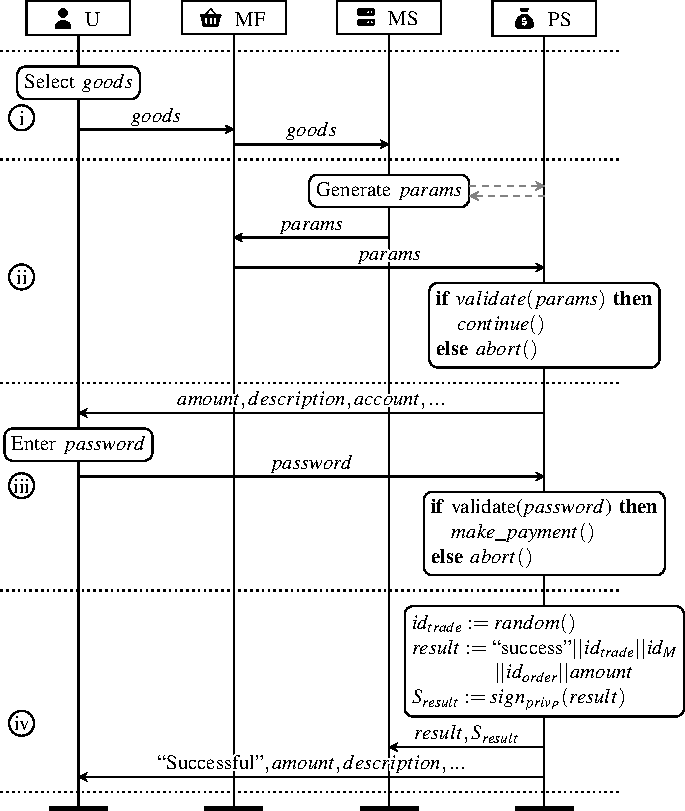
\includegraphics[width=\linewidth]{img/tpp_process.pdf}
%DIFDELCMD <     %%%
\DIFdelendFL \DIFaddbeginFL 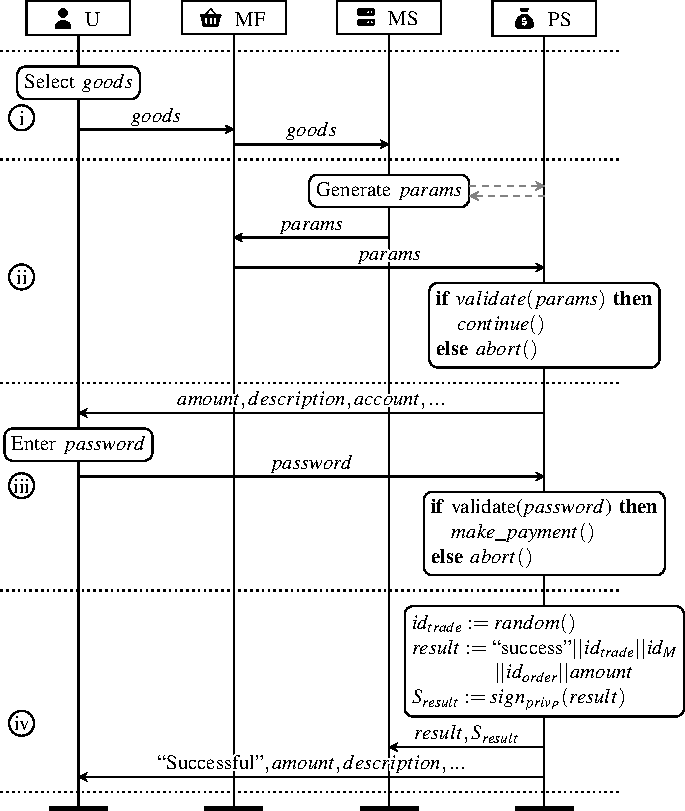
\includegraphics[width=0.85\linewidth]{img/tpp_process.pdf}
    \DIFaddendFL \caption{
        An Overview of a Typical Third-Party Online Payment. 
        Dashed arrows indicate optional messages, depending on the specific payment pattern.
        Notation: $validate(p)$ denotes checking whether $p$ is valid; $continue()$ denotes continuing the execution of the protocol; $abort()$ denotes terminating the protocol; $make\_payment()$ denotes the fund transfer operation; $random()$ denotes generating a random number; and $sign_k(m)$ denotes signing message $m$ with key $k$.
    }
    \label{fig:third_party_payment}
\end{figure}

\subsection{Payment Patterns}\label{sec:payment-models}
During the \emph{Prepayment} phase, the generation methods of payment parameters vary across different providers and scenarios.
We introduce two high-level payment patterns adopted by the two leading payment providers, PSP-B and Alipay.

\DIFdelbegin %DIFDELCMD < \begin{figure}[t]
%DIFDELCMD <   %%%
\DIFdelendFL \DIFaddbeginFL \begin{figure*}[t]
  \DIFaddendFL \centering
  \DIFaddbeginFL \begin{minipage}[b]{0.48\textwidth}
    \centering
    \DIFaddendFL 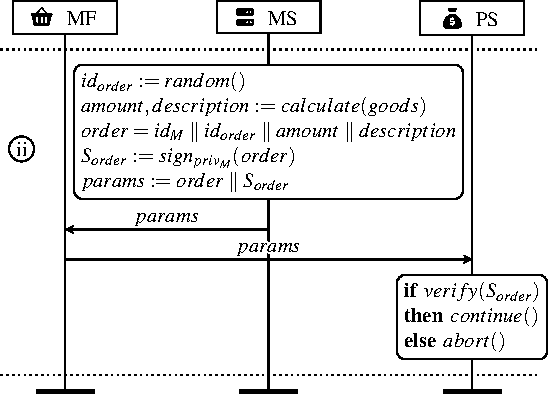
\includegraphics[width=0.9\linewidth]{img/model_a.pdf}
    \caption{Payment Pattern A}
    \label{fig:payment_model_a}
  \DIFdelbeginFL %DIFDELCMD < \end{figure}
%DIFDELCMD < 

%DIFDELCMD < \begin{figure}[t]
%DIFDELCMD <   %%%
\DIFdelendFL \DIFaddbeginFL \end{minipage}
  \hfill
  \begin{minipage}[b]{0.48\textwidth}
    \DIFaddendFL \centering
    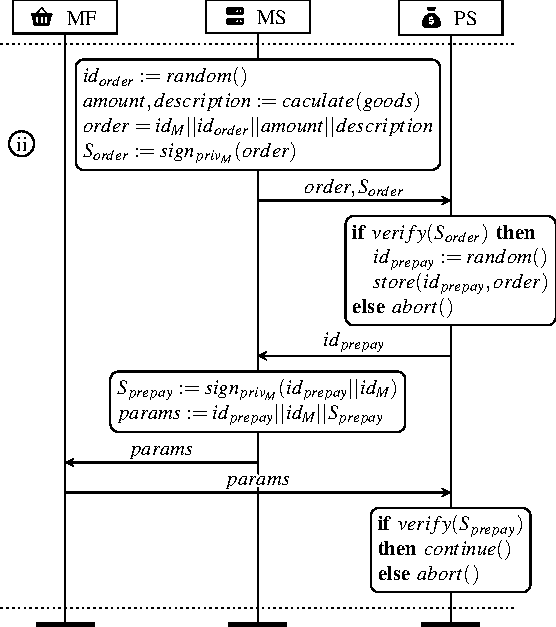
\includegraphics[width=0.9\linewidth]{img/model_b.pdf}
    \caption{Payment Pattern B}
    \label{fig:payment_model_b}
  \DIFdelbeginFL %DIFDELCMD < \end{figure}
%DIFDELCMD < %%%
\DIFdelend \DIFaddbegin \end{minipage}
\end{figure*}
\DIFaddend 

\textbf{Payment Pattern A.}
In this pattern, the payment parameters are generated directly by the \emph{MS}.
Fig\DIFdelbegin \DIFdel{ure}\DIFdelend  .~\ref{fig:payment_model_a} details the process by which the \emph{MS} generates the \emph{order information}.
Based on the $goods$ selected by the user, the \emph{MS} calculates the $amount$ to be paid and the order $description$, and generates a unique order identifier~($id_{order}$). 
These values, together with the merchant identifier~($id_{M}$), constitute the order information.
The \emph{MS} then signs the order information using its private key $priv_{M}$, producing a signature value $S_{order}$.
The order information and $S_{order}$ are used directly as the payment parameters.
The \emph{PS} then verifies $S_{order}$ to ensure the integrity of the order information.
Payment pattern A is employed by Alipay in the in-app and mobile web payment scenarios.

\textbf{Payment Pattern B.}
In this pattern, the payment parameters are generated by the \emph{MS} with the involvement of the \emph{PS}.
% Similarly, the \emph{MS} is required to sign the critical order information.
As in pattern~A, the \emph{MS} must sign the critical order information.
However, unlike pattern~A, the order information and its signature, $S_{order}$, cannot be used directly as payment parameters.
Instead, they are sent to the \emph{PS} as a prepayment request.
After verifying $S_{order}$, the \emph{PS} generates a unique prepayment identifier, $id_{prepay}$, for the payment and returns it to the \emph{MS}.
The \emph{MS} then concatenates $id_{M}$ with $id_{prepay}$ and signs the result using $priv_{M}$, producing the signature $S_{prepay}$.
Finally, $id_{M}$, $id_{prepay}$ and $S_{prepay}$ are sent to the \emph{PS} as the payment parameters.
The \emph{PS} verifies the validity of $S_{prepay}$ to ensure the integrity of the payment request.
Payment pattern~B is adopted by Alipay in the QR Code Payment scenario and by PSP-B across all three payment scenarios.


\subsection{\Tamarin}

\Tamarin is a symbolic verification tool widely used for analyzing real-world security protocols, including 
EMV~\cite{Radu2022EMVRelayProtection,Basin2021EMVStandard,Basin2021CardBrandMixup}, 
TLS~\cite{Cremers2016AutomatedTLS,Cremers2017ComprehensiveTLS,Lee2019maTLS}, 
Bluetooth~\cite{Shi2023FormalBLEPairing,Jangid2023ExtrapolatingBluetoothPasskey}, 
and 5G-AKA~\cite{basin2018formal,cremers2019component}.
It employs a multiset rewriting system to model both protocol execution and adversary capabilities, providing a rich language for specifying security properties as first-order logic formulas over execution traces. 
\Tamarin supports unbounded protocol sessions, a Dolev-Yao style adversary, and is particularly well-suited for analyzing stateful protocols due to its native handling of mutable and persistent state.

\DIFdelbegin \textbf{\DIFdel{Terms and Facts.}}
%DIFAUXCMD
\DIFdel{In }\DIFdelend \Tamarin \DIFdelbegin \DIFdel{, protocol messages are represented }\DIFdelend \DIFaddbegin \DIFadd{represents messages }\DIFaddend as \emph{terms} \DIFdelbegin \DIFdel{, which are constructed from variables, constants, and compound expressions formed by applying function symbols to subterms.
An equational theoryover terms specifies algebraic properties and reducibility relations, thereby affecting pattern matching and substitution.
For example, symmetric encryption is modeled by a encryption function $\text{\Tfunction{senc}}$ and a decryption function $\text{\Tfunction{sdec}}$ satisfying the equation $\text{\Tfunction{sdec}}(\text{\Tfunction{senc}}(m,k),k)=m$.
The system state is captured using }\DIFdelend \DIFaddbegin \DIFadd{built from function symbols under an equational theory, and the system state as a multiset of }\DIFaddend \emph{facts} \DIFdelbegin \DIFdel{, which are predicates of the form }\DIFdelend \TFactTerm{F}{$t_1,\ldots,t_n$}.
\DIFdelbegin \DIFdel{Facts can be linear (consumed upon rule application), persistent (available throughout the execution, e.g., }%DIFDELCMD < \TFactTerm{!PK}{$A,Pk_A$}%%%
\DIFdel{).
The system execution can be observed using action facts, which record execution steps such as }%DIFDELCMD < \TFactTerm{Running}{$A,x$} %%%
\DIFdel{and }%DIFDELCMD < \TFactTerm{Commit}{$B,x$} %%%
\DIFdel{and are retained to form execution traces but do not constitute system states.
}%DIFDELCMD < 

%DIFDELCMD < %%%
\textbf{\DIFdel{Multiset Rewriting Rules.}}
%DIFAUXCMD
\DIFdel{Multiset rewriting rules formally describe protocol behavior.
Each rule specifies a state transition by means of }\emph{\DIFdel{left-hand side}} %DIFAUXCMD
\DIFdel{premise facts (guards) and }\emph{\DIFdel{right-hand side}} %DIFAUXCMD
\DIFdel{conclusion facts (productions), and may also include action facts as observable events.
Formally, a rule can be written as following:
}%DIFDELCMD < \begin{tightflalign}
%DIFDELCMD <   \TFacts{  LF_1,\ldots,LF_m } \TActFactsSL{AF(t_1, \ldots, t_k)} \TFacts{  RF_1, \ldots, RF_n } &
%DIFDELCMD < \end{tightflalign}
%DIFDELCMD < %%%
\DIFdel{Given a current state multiset $S$, the rule }\DIFdelend \DIFaddbegin \DIFadd{Linear facts are consumed when a rule uses them, while persistent facts, written with a leading ``!'', remain available.
A multiset rewriting rule $\TFacts{L} \TActFactsSL{A} \TFacts{R}$ }\DIFaddend is enabled when \DIFdelbegin \DIFdel{$LF_1,\ldots,LF_m \subseteq S$.
We use the function }%DIFDELCMD < \funcText{linear} %%%
\DIFdel{to denotes }\DIFdelend \DIFaddbegin \DIFadd{its premises $L$ are in the state; it consumes }\DIFaddend the linear facts \DIFdelbegin \DIFdel{from a set of facts.
The application of the rule produces a new state $S' = (S \setminus \text{\funcText{linear}}(\{LF_1,\ldots,LF_m\})) \cup \{RF_1, \ldots, RF_n\}$, and appends }\DIFdelend \DIFaddbegin \DIFadd{in $L$, adds the conclusions $R$, and records }\DIFaddend the action facts \DIFdelbegin \DIFdel{$AF(t_1, \ldots, t_k)$ to }\DIFdelend \DIFaddbegin \DIFadd{$A$ in }\DIFaddend the execution trace.
\DIFdelbegin %DIFDELCMD < 

%DIFDELCMD < %%%
\textbf{\DIFdel{Trace and Formulas.}}
%DIFAUXCMD
\DIFdel{In }%DIFDELCMD < \Tamarin%%%
\DIFdel{, the global behavior of a protocol is captured by traces, which are sequences of action facts .
Formally, a trace is represented as $\tau = \langle FA_1@t_1, FA_2@t_2, \dots, FA_n@t_n \rangle$, where $FA_i@t_i$ denotes an observable event occurring at time point $t_i$.
Based on such traces, }%DIFDELCMD < \Tamarin %%%
\DIFdel{reasons about executions using }\DIFdelend \DIFaddbegin \DIFadd{Security properties (lemmas) are }\DIFaddend first-order \DIFdelbegin \DIFdel{logic formulas, where }\emph{\DIFdel{restrictions}} %DIFAUXCMD
\DIFdel{are used to specify global constraints over all possible executions.
These constraints are also first-order logic formulas over events and time points.
Within this restricted semantic space, security properties are likewise expressed as first-order temporal logic formulas (lemmas), such as secrecy, authentication, or consistency properties, and are required to hold for all valid traces.
For example, key secrecy can be formalized as:
}%DIFDELCMD < \begin{tightflalign}
%DIFDELCMD <     \TAll %%%
\DIFdel{\;\text{\Tterm{k \#i.}} \;\text{\TFact{Install(k)@\#i}} }%DIFDELCMD < \implies \TNot %%%
\DIFdel{(}%DIFDELCMD < \TEx %%%
\DIFdel{\;\, \text{\TLemma{\#j.}} \;\text{\TFact{K(k)@\#j}} ) 
}%DIFDELCMD < \end{tightflalign}
%DIFDELCMD < %%%
\DIFdel{This formula expresses that for any key $k$ and time point $i$, if this key~$k$ is installed at time~$i$, then there doesn't exist a time point~$j$ at which the key~$k$ is known by an adversary.
}\DIFdelend \DIFaddbegin \DIFadd{formulas over the action facts of a trace and their time points, and restrictions use the same language to exclude executions.
}\DIFaddend 

%-------------------------------------------------------------------------------
\section{Threat Model and Assumptions}
%-------------------------------------------------------------------------------

In this section, we introduce the threat model and security assumptions used in our formal analysis and attacks.

\subsection{Threat Model}
\DIFdelbegin \DIFdel{In this paper, we consider the following adversary model.
}\DIFdelend 

\begin{enumerate}[leftmargin=*]
  \item \textbf{Payment Parameter Acquisition.}
  We assume that \DIFaddbegin \DIFadd{the }\DIFaddend adversary can obtain legitimate payment parameters for arbitrary goods from any merchant platform.
  This assumption is realistic, as most merchant platforms support public registration, allowing adversaries to create accounts and complete purchases to acquire payment parameters.
  \item \textbf{Compromised Insecure Channels.}
  The adversary follows the standard Dolev-Yao model, where the adversary is able to fully control insecure communication channels, including eavesdropping, modifying, replaying, and injecting arbitrary messages.
  In third-party online payment ecosystems, \emph{PS} cannot provide absolute security guarantees for all communication channels between external entities. 
  Therefore, we adopt weak assumptions for such external channels and grant the adversary man-in-the-middle capabilities over these insecure channels. 
  % We will discuss which channels are considered insecure in Section~\ref{sec:security_assumptions}.
  The specific channels considered insecure are discussed in Section~\ref{sec:security_assumptions}.
\end{enumerate}



\subsection{Security Assumptions} \label{sec:security_assumptions}

Regarding the user, the payment system, and the communication channel, we make the following security assumptions:

\textbf{User Assumptions.}
During the \emph{Authorization} phase, users review the order information before authorizing the payment.
We assume that users can correctly verify whether the payment \emph{amount} and order \emph{description} displayed by the \emph{PS-App} match the goods selected on the \emph{MF}.
Another key element displayed on the payment interface is the payee's account name. 
However, since this name does not necessarily correspond to the merchant's brand name, \emph{U} cannot reliably verify whether the displayed account belongs to the intended merchant.
For instance, when purchasing a video game on Steam (a leading global digital game distribution and social platform), the payee's name shown is ``Valve Corporation'' (the parent company of Steam) rather than ``Steam''.
Users without relevant background knowledge may find it difficult to determine whether ``Valve Corporation'' is indeed the payee account associated with ``Steam''.
Therefore, we assume that users do not rely on the payee's account name when \DIFaddbegin \DIFadd{authorizing a payment.
}\DIFaddend 

\textbf{Payment System Assumptions.}
The \emph{PS} comprises two components: the \emph{PS-App} and the \emph{PS-Server}.  
We assume that the \emph{PS-App} and the \emph{PS-Server}, as well as the communication channel between them, are trusted. 
Unless otherwise specified, we treat them as a single \emph{PS} entity in the subsequent analysis.

\textbf{Channel Assumptions.}
According to developer manuals of various payment providers, the \emph{MS} is recommended to be configured with security protocols such as HTTPS to ensure secure communication. 
This implies that channels where \emph{MS} participates should be secure.
However, we note that this assumption is overly strict, as a recommendation in the developer manual alone cannot provide a reliable guarantee of secure communication. 
Therefore, in our analysis, we relax the security assumptions for certain channels.
We consider the following communication channels to be potentially insecure:
\begin{enumerate}[leftmargin=*]
\item[\Rom{1}.] \textbf{\emph{MF} $\Longleftrightarrow$ \emph{MS}:}
  We assume that the channel between \emph{MF} and \emph{MS} is insecure.
  This assumption is motivated by the fact that \emph{MF} operates on the user's device, and users should not be assumed to possess a high level of security awareness or to be able to defend against diverse threats in real-world network environments.
  In addition, given the large number of merchants involved, payment service providers cannot guarantee that all front-end and back-end communications of merchants are free from security vulnerabilities.
\item[\Rom{2}.] \textbf{\emph{MF} $\Longleftrightarrow$ \emph{PS}:}
  The communication between \emph{MF} and \emph{PS} occurs during the \emph{Prepayment} phase, in which \emph{MF} invokes the \emph{PS-App} to send payment parameters.
  This interaction is vulnerable to hijacking attacks in practice, as evidenced by real-world exploits discussed in Section~\ref{sec:real_world}.
  Thus, we assume that this channel is insecure.
\end{enumerate}


%-------------------------------------------------------------------------------
\section{Payment Protocol Modeling} \DIFaddbegin \label{sec:modeling}
\DIFaddend %-------------------------------------------------------------------------------
We formally model the payment protocols of PSP-B and Alipay in three payment scenarios, and the full models are available in an open-source repository~\cite{third_payment_model_2026}.
In this section, we present the key details for modeling third-party payment protocols.
First, we describe the user model, which allows us to capture users' evaluation of payment information and their authorization behavior within the symbolic model.
Then, we introduce the oracle model for the adversary to obtain legitimate payment parameters.

% \subsection{Channel Model}
% We introduce appropriate modifications to the standard secure channel model in order to systematically model different channels and security assumptions.
% We use the facts \TFact{SOut} and \TFact{SIn} to represent message sending and receiving over a channel.
% Messages transmitted over our secure channels are not replayable.
% Therefore, the message transmission process of the channel is simplified, and the rule is shown below.
% \begin{tightflalign}
% \text{\Tterm{Ru}}  & \text{\Tterm{le SecureChannel}} :      & \\
%   \TFacts{  & \text{\TFactTerm{SOut}{ChannelID, A, B, m}}}  \\
%             & \TEmpActFactSL{}                                \\
%   \TFacts{  & \text{\TFactTerm{SIn}{ChannelID, A, B, m}}}
% \end{tightflalign}
% Here, \Tterm{m} is the message transmitted over the channel, \Tterm{A} denotes the message sender, and \Tterm{B} denotes the message receiver.
% \Tterm{ChannelID} is a channel identifier that specifies which channel is used for communication.
% For example, when \Tterm{ChannelID} takes the value \Tterm{\textquotesingle U-PS\textquotesingle}, it denotes the communication channel between \emph{U} and \emph{PS}.

% To model insecure channels, we introduce two additional attack rules for such channels, corresponding to violations of channel confidentiality and integrity, respectively.
% \begin{tightflalign}
% \text{\Tterm{Ru}}  & \text{\Tterm{le BreakConfidentiality}} :                   & \\
%   \TFacts{  & \text{\TFactTerm{SOut}{ChannelID, A, B, m}} }                     \\
%             & \TActFactsSL{ \text{\TFactTerm{InsecureChannel}{ChannelID}}}      \\
%   \TFacts{  & \text{\TFactTerm{SOut}{ChannelID, A, B, m}, \TFactTerm{Out}{m}}}  \\ \\
% \text{\Tterm{Ru}}  & \text{\Tterm{le BreakIntegrity}} :                         \\
%   \TFacts{  & \text{\TFactTerm{In}{\TPairN{ChannelID, A, B, m}}} }              \\
%             & \TActFactsSL{ \text{\TFactTerm{InsecureChannel}{ChannelID}}}      \\
%   \TFacts{  & \text{\TFactTerm{SOut}{ChannelID, A, B, m}}}                      
% \end{tightflalign}
% Compromising confidentiality grants the adversary the ability to obtain messages from the channel, while compromising integrity grants the adversary the ability to inject arbitrary messages into the channel.
% \TFact{In} and \TFact{Out} are built-in facts of the Tamarin prover that represent receiving messages from, and sending messages to, the public channel.
% The fact \TFact{InsecureChannel} is used to label a channel as insecure. 
% We use a restriction to constrain the adversary so that it can compromise only the channels specified under a given channel assumption.
% \begin{tightflalign}
% \text{\Tterm{Re}}  & \text{\Tterm{striction Insecure}} :            & \\
%     & \TAll \; \text{\Tterm{ch\_id k \#i.}} \; \text{\TFact{InsecureChannel(ch\_id)@\#i}} \\
%     & \implies (\text{\Tterm{ch\_id}} = \text{\Tterm{\textquotesingle MF-MS\textquotesingle}} \; \lor \; \text{\Tterm{ch\_id}} = \text{\Tterm{\textquotesingle MF-PS\textquotesingle}} ) 
% \end{tightflalign}
% This restriction specifies that the channels between \emph{MF} and \emph{MS}, and between \emph{MF} and \emph{PS}, are insecure.

\subsection{User Model} 
Under our security assumptions, users are capable of accurately identifying the payment $amount$ and $description$, thereby avoiding being misled into authorizing a payment.
To model this capability in the symbolic model, we introduce two unary functions, 
\Tfunction{calc\_amt} and \Tfunction{gen\_desc}, which are used to compute the payment $amount$ and $description$ from $goods$, respectively.
During the \emph{Order\DIFdelbegin \DIFdel{ing}\DIFdelend  } phase, users select goods.
For the same goods (note that this does not refer to the same product model), a user can only purchase them at most once. 
Therefore, in our model, we use a fresh value as an abstract representation of the goods.
The following rule models the user's goods ordering behavior:
\begin{tightflalign}
      \TFacts{ \text{\TFact{Fr}}(\TSymbolFr goods)} \TEmpActFactSL{}  
      \TFacts{
        \text{\TFact{Order}}(\TSymbolFr goods),
        \text{\TFact{SOut}}(..., \TSymbolFr goods)
      }
\end{tightflalign}
This rule represents that the user \emph{U} selects a product $\TSymbolFr goods$ and sends it to \emph{MF}.
Here, $\text{\TFact{Fr}}(\TSymbolFr goods)$ indicates that the value $\TSymbolFr goods$ is freshly generated.
$\text{\TFact{Order}}(\TSymbolFr goods)$ indicates that the user has placed an order for the goods $\TSymbolFr goods$.
In \DIFaddbegin \DIFadd{the }\DIFaddend \emph{Prepayment} phase, \emph{MS} computes the payment $amount$ and $description$ based on $\TSymbolFr goods$ using \Tfunction{calc\_amt} and \Tfunction{gen\_desc}, as follows:
\begin{tightflalign}
      amount & = \text{\Tfunction{calc\_amt}}(\TSymbolFr goods) &\\
      description & = \text{\Tfunction{gen\_desc}}(\TSymbolFr goods)
\end{tightflalign}
In \DIFaddbegin \DIFadd{the }\DIFaddend \emph{Authorization} phase, the user obtains the order information from the \emph{PS-App} and confirms it.
Due to pattern matching, the user authorizes a payment if \DIFaddbegin \DIFadd{and }\DIFaddend only if the payment $amount$ and $description$ exactly match $\text{\Tfunction{calc\_amt}}(\TSymbolFr goods)$ and $\text{\Tfunction{gen\_desc}}(\TSymbolFr goods)$, respectively, and will not authorize any other values.
The following rule models the user's payment authorization behavior:
\begin{tightflalign}
      \TFacts{ &\text{\TFact{Order}}(\TSymbolFr goods),                     &\\
              &\text{\TFact{SIn}}(..., \TPair{\text{\Tfunction{calc\_amt}}(\TSymbolFr goods), \text{\Tfunction{gen\_desc}}(\TSymbolFr goods)}) } \\
      & \TEmpActFactSL{} 
      \TFacts{ \text{\TFact{UserAuthorizePayment}}(...) }
\end{tightflalign}
Here, \TFact{UserAuthorizePayment} indicates that the user authorizes the payment.
Notably, the above model implies that users can accurately distinguish between different items, even when they belong to the same product model.
In practice, users do not possess such capabilities, nor do merchant platforms provide functionality that allows users to select items based on product serial numbers.
Nevertheless, this idealized user model helps us focus on analyzing the security of the payment protocol itself, without conflating the analysis with errors that users may make.

\subsection{Adversarial Capabilities Model}
In our threat model, the adversary is capable of obtaining legitimate payment parameters.
In practice, the adversary acquires such legitimate payment parameters by accessing merchant platforms in a normal manner and placing orders to purchase goods.
To intuitively model this behavior, we introduce an \emph{Order Oracle} within the symbolic framework, which is defined by the following rule:
\begin{tightflalign}
\text{\Tterm{Ru}}  & \text{\Tterm{le OrderOracle}} :        & \\
  \TFacts{  & \text{\TFactTerm{In}{<$amt$, $desc$>}, \TFactTerm{!Merchant}{$id_M$, $priv_M$}}} 
             \TEmpActFactSL{}                              \\
  \TFacts{  & \text{\TFactTerm{Out}{\text{\Tfunction{gen\_params($amt$, $desc$, $id_M$, $priv_M$)}}}}}
\end{tightflalign}
By querying this oracle with an order amount $amt$ and an order description $desc$, the adversary can obtain the corresponding legitimate payment parameters.
The oracle is granted access to the merchant's identifier $id_M$ and \DIFaddbegin \DIFadd{p}\DIFaddend rivate key $priv_M$, enabling it to generate legitimate payment parameters that are accepted by \emph{PS}.
The function \Tfunction{gen\_params($amt$, $desc$, $id_M$, $priv_M$)} represents the process by which the oracle generates payment parameters from $amt$ and $desc$.
This process is consistent with the procedure used by merchants to generate payment parameters in both payment pattern~A and payment pattern~B.
We use equations to flexibly define this process in symbolic models.
In protocols conforming to \DIFdelbegin \DIFdel{Model}\DIFdelend \DIFaddbegin \DIFadd{pattern}\DIFaddend ~A, the equation is defined as follows:
\begin{tightflalign}
  \text{\Tfunction{gen\_par}} & \text{\DIFdelbegin %DIFDELCMD < \Tfunction{mas}%%%
\DIFdelend \DIFaddbegin \Tfunction{ams}\DIFaddend }(amt, desc, id_M, priv_M) = \\
  & amt \parallel desc \parallel id_M \parallel \text{\Tfunction{sign}}(amt \parallel desc \parallel id_M, priv_M)
\end{tightflalign}
For protocols under \DIFdelbegin \DIFdel{Model}\DIFdelend \DIFaddbegin \DIFadd{pattern}\DIFaddend ~B, the equation is as follows:
\begin{tightflalign}
  \text{\DIFdelbegin %DIFDELCMD < \Tfunction{gen\_parmas}%%%
\DIFdelend \DIFaddbegin \Tfunction{gen\_params}\DIFaddend }(am&t, desc, id_M, priv_M, id_{prepay})   = \\
  & id_{prepay} \parallel id_M \parallel \text{\Tfunction{sign}}(id_{prepay} \parallel id_M, priv_M)
\end{tightflalign}
Here, our equation simplifies the actual generation process of payment parameters, such as the generation of $id_{prepay}$.
In the modeling, we incorporate additional necessary parameters and computational steps according to the details of the actual protocol, ensuring the model's accuracy and completeness.

%-------------------------------------------------------------------------------
\section{Security Properties} \label{sec:security_properties}
%-------------------------------------------------------------------------------

In this section, we formally define the security properties of third-party online payment protocols.
The core security goal of protocols is to ensure that the user, the merchant, and the payment service provider reach a consistent view of a transaction.
The protocol must guarantee that (a) all parties agree on the payment order being processed, (b) each payment is authorized by the user, and (c) the reported payment result faithfully reflects the actual fund transfer.

All properties considered in this section are instances of \emph{injective agreement}~\cite{Lowe1997AuthenticationHierarchy}.
Injective agreement strengthens standard agreement by requiring a one-to-one correspondence between protocol runs: 
each successful local completion must correspond to a unique execution of the peer, ruling out replay, duplication, or reuse of protocol messages.
Two types of atomic facts are necessary to define injective agreement:
\begin{enumerate}[leftmargin=*]
  \item $\mathsf{Running}(A,B,x)$: 
    records that party $A$ is interacting with $B$ in a concrete execution of the protocol and that the interaction involves data $x$ (an objective execution fact);
  \item $\mathsf{Commit}(A,B,x)$:
    denotes that party $A$ subjectively believes that it has reached agreement with $B$ on data $x$ (e.g., after receiving and accepting a message).
\end{enumerate}
\DIFdelbegin \DIFdel{This notion is particularly well-suited for online payment scenarios, where both consistency and uniqueness of transactions are fundamentally essential requirements.
}\DIFdelend We structure the security properties according to the logical progression of a payment protocol, namely agreement on the \emph{order}, agreement on \emph{user authorization}, and agreement on the \emph{result}.

\DIFdelbegin \subsection{\DIFdel{Injective Agreement on Order}}
%DIFAUXCMD
\addtocounter{subsection}{-1}%DIFAUXCMD
\DIFdelend \DIFaddbegin \DIFadd{Each property instantiates the following template, in which $\mathsf{Commit}$ and $\mathsf{Running}$ are replaced by the fact pair of that property:
}\begin{tightflalign}
  \TAll \DIFadd{\; \text{\Tterm{a}} }& \DIFadd{\text{\Tterm{ b x \#i.}} \; \text{\TFact{Commit(a, b, x)@\#i}} }&\\
  \implies & \TEx \DIFadd{\; \text{\TLemma{\#j.}} \; \text{\TFact{Running(b, a, x)@\#j}} }\land \DIFadd{\text{\Tterm{\#j < \#i}} }\land\\
  \lnot \DIFadd{\; }&\DIFadd{(\;}\TEx \DIFadd{\; \text{\TLemma{a2 b2 \#i2.}} \; \text{\Tterm{\#i2}} \neq \text{\Tterm{\#i}} \; }\land\\
  & \DIFadd{\hspace{2em} \text{\TFact{Commit(a2, b2, x)@\#i2}})
}\end{tightflalign}
\DIFadd{The first conjunct requires that the peer actually ran the protocol on the same data, and the second requires that no other commit uses that data, which rules out replay and duplication.
The Commit and Running facts follow the standard interpretation introduced in~\mbox{%DIFAUXCMD
\cite{Lowe1997AuthenticationHierarchy}}\hskip0pt%DIFAUXCMD
.
}\DIFaddend 

\DIFdelbegin \DIFdel{Injective agreement on the order }\DIFdelend \DIFaddbegin \textbf{\DIFadd{Injective Agreement on Order.}}
\DIFadd{This property }\DIFaddend ensures that all involved parties process the same payment order and that each order is handled at most once\DIFdelbegin \DIFdel{.
Violations of this property indicate }\DIFdelend \DIFaddbegin \DIFadd{; a violation indicates }\DIFaddend that an adversary \DIFdelbegin \DIFdel{may have }\DIFdelend \DIFaddbegin \DIFadd{has }\DIFaddend tampered with the order information\DIFdelbegin \DIFdel{or caused inconsistent views among the participants.
Since this property }\DIFdelend \DIFaddbegin \DIFadd{.
Since it }\DIFaddend involves three principals, we \DIFdelbegin \DIFdel{separately consider the agreements between }\DIFdelend \DIFaddbegin \DIFadd{consider }\DIFaddend \emph{PS} and \emph{MS}, and \DIFdelbegin \DIFdel{between }\DIFdelend \emph{U} and \emph{MS}\DIFdelbegin \DIFdel{.
}%DIFDELCMD < 

%DIFDELCMD < %%%
\textbf{\DIFdel{IA-O1~(}\emph{\DIFdel{PS}} %DIFAUXCMD
\DIFdel{$\leftarrow$ }\emph{\DIFdel{MS}}%DIFAUXCMD
\DIFdel{):}} 
%DIFAUXCMD
\DIFdel{This lemma captures injective agreement on the order from the perspective of }\DIFdelend \DIFaddbegin \DIFadd{, separately.
}\emph{\DIFadd{IA-O1~(}\emph{\DIFadd{PS}} \DIFadd{$\leftarrow$ }\emph{\DIFadd{MS}}\DIFadd{)}} \DIFadd{uses }\TFact{PSCommit(ps, ms, order)} \DIFadd{and }\TFact{MSRunning(ms, ps, order)}\DIFadd{: if }\DIFaddend \emph{PS} \DIFdelbegin \DIFdel{.
If }\emph{\DIFdel{PS}} %DIFAUXCMD
\DIFdelend accepts a payment request for an order allegedly issued by \emph{MS}, then \emph{MS} \DIFdelbegin \DIFdel{must have previously initiated a corresponding }\DIFdelend \DIFaddbegin \DIFadd{has initiated a }\DIFaddend request for that order\DIFdelbegin \DIFdel{.
Moreover, no other payment }\DIFdelend \DIFaddbegin \DIFadd{, and no other }\DIFaddend request for the same order \DIFdelbegin \DIFdel{can be accepted by }\emph{\DIFdel{PS}}%DIFAUXCMD
\DIFdel{, ensuring uniqueness.
The property is formalized as follows:
}%DIFDELCMD < \begin{tightflalign}
%DIFDELCMD <   \TAll %%%
\DIFdel{\; \text{\Tterm{ps}} }%DIFDELCMD < & %%%
\DIFdel{\text{\Tterm{ ms order \#i.}} \; \text{\TFact{PSCommit(ps, ms, order)@\#i}} }%DIFDELCMD < &\\
%DIFDELCMD <   \implies & \TEx %%%
\DIFdel{\; \text{\TLemma{\#j.}} \; \text{\TFact{MSRunning(ms, ps, order)@\#j}} \; }%DIFDELCMD < \land\\
%DIFDELCMD <   \lnot %%%
\DIFdel{\; }%DIFDELCMD < &%%%
\DIFdel{(\;}%DIFDELCMD < \TEx %%%
\DIFdel{\; \text{\TLemma{ps2 ms2 \#i2.}} \; \text{\Tterm{\#i2}} \neq \text{\Tterm{\#i}} \; }%DIFDELCMD < \land\\
%DIFDELCMD <   & %%%
\DIFdel{\hspace{2em} \text{\TFact{PSCommit(ps2, ms2, order)@\#i2}}) 
}%DIFDELCMD < \end{tightflalign}
%DIFDELCMD < %%%
\DIFdel{Here, the }\emph{\DIFdel{Commit}} %DIFAUXCMD
\DIFdel{and }\emph{\DIFdel{Running}} %DIFAUXCMD
\DIFdel{facts follow the standard interpretation introduced in~\mbox{%DIFAUXCMD
\cite{Lowe1997AuthenticationHierarchy}}\hskip0pt%DIFAUXCMD
.
The fact }%DIFDELCMD < \TFact{PSCommit(ps, ms, order)} %%%
\DIFdel{denotes that }\emph{\DIFdel{PS}} %DIFAUXCMD
\DIFdel{has accepteda payment request for }%DIFDELCMD < \Tterm{order}%%%
\DIFdel{, 
while }%DIFDELCMD < \TFact{MSRunning(ms, ps, order)} %%%
\DIFdel{records that }\emph{\DIFdel{MS}} %DIFAUXCMD
\DIFdel{has actually issued such a request}\DIFdelend \DIFaddbegin \DIFadd{is accepted}\DIFaddend .
The term \Tterm{order} \DIFdelbegin \DIFdel{denotes order information, including }\DIFdelend \DIFaddbegin \DIFadd{includes }\DIFaddend the merchant's order identifier, the payment amount, and the product description.
\DIFdelbegin %DIFDELCMD < 

%DIFDELCMD < %%%
\textbf{\DIFdel{IA-O2~(}\emph{\DIFdel{U}} %DIFAUXCMD
\DIFdel{$\leftarrow$ }\emph{\DIFdel{MS}}%DIFAUXCMD
\DIFdel{):}} 
%DIFAUXCMD
\DIFdel{From the user 's perspective, injective agreement on the order ensures that the user }\DIFdelend \DIFaddbegin \emph{\DIFadd{IA-O2~(}\emph{\DIFadd{U}} \DIFadd{$\leftarrow$ }\emph{\DIFadd{MS}}\DIFadd{)}} \DIFadd{uses }\TFact{UMCommit(u, ms, goods)} \DIFaddend and \DIFaddbegin \TFact{MSRunning(ms, u, goods)}\DIFadd{: the user and }\DIFaddend the merchant \DIFdelbegin \DIFdel{reach agreement on order information during the payment process, and that }\DIFdelend \DIFaddbegin \DIFadd{agree on the purchased goods, and }\DIFaddend each order is processed exactly once.
\DIFdelbegin \DIFdel{The formalization is as follows:
}%DIFDELCMD < \begin{tightflalign}
%DIFDELCMD <   \TAll %%%
\DIFdel{\; \text{\Tterm{u }} }%DIFDELCMD < & %%%
\DIFdel{\text{\Tterm{ms goods \#i.}} \; \text{\TFact{UMCommit(u, ms, goods)@\#i}} }%DIFDELCMD < &\\
%DIFDELCMD <   \implies & \TEx %%%
\DIFdel{\; \text{\TLemma{\#j.}} \; \text{\TFact{MSRunning(ms, u, goods)@\#j}} \; }%DIFDELCMD < \land\\
%DIFDELCMD <   \lnot %%%
\DIFdel{\; }%DIFDELCMD < &%%%
\DIFdel{(\;}%DIFDELCMD < \TEx %%%
\DIFdel{\; \text{\TLemma{u2 ms2 \#i2.}} \; \text{\Tterm{\#i2}} \neq \text{\Tterm{\#i}} \; }%DIFDELCMD < \land\\
%DIFDELCMD <   & %%%
\DIFdel{\hspace{2em} \text{\TFact{UMCommit(u2, ms2, goods)@\#i2}}) 
}%DIFDELCMD < \end{tightflalign}
%DIFDELCMD < %%%
\DIFdel{Unlike the order information considered in IA-O1, }\DIFdelend IA-O2 \DIFdelbegin \DIFdel{only requires agreement between the user and the merchant on the purchased goods }\DIFdelend \DIFaddbegin \DIFadd{requires agreement on the goods only}\DIFaddend , since the user is primarily concerned with what is being bought.

\DIFdelbegin \subsection{\DIFdel{Injective Agreement on User Authorization}}
%DIFAUXCMD
\addtocounter{subsection}{-1}%DIFAUXCMD
%DIFDELCMD < 

%DIFDELCMD < %%%
\DIFdel{Injective agreement on user authorization }\DIFdelend \DIFaddbegin \textbf{\DIFadd{Injective Agreement on User Authorization.}}
\DIFadd{This property }\DIFaddend ensures that each successful payment is backed by a unique and explicit authorization from the user\DIFdelbegin \DIFdel{.
This property }\DIFdelend \DIFaddbegin \DIFadd{, which }\DIFaddend prevents both unauthorized payments and \DIFdelbegin \DIFdel{reuse of a single authorization to complete }\DIFdelend \DIFaddbegin \DIFadd{the reuse of one authorization for }\DIFaddend multiple transactions.
\DIFdelbegin %DIFDELCMD < 

%DIFDELCMD < %%%
\textbf{\DIFdel{IA-UA~(}\emph{\DIFdel{PS}} %DIFAUXCMD
\DIFdel{$\leftarrow$ }\emph{\DIFdel{U}}%DIFAUXCMD
\DIFdel{):}}
%DIFAUXCMD
\DIFdel{Specifically, }\DIFdelend \DIFaddbegin \emph{\DIFadd{IA-UA~(}\emph{\DIFadd{PS}} \DIFadd{$\leftarrow$ }\emph{\DIFadd{U}}\DIFadd{)}} \DIFadd{uses }\TFact{PaymentComplete(u, h(p), s)} \DIFadd{and }\TFact{UserInputPwd(u, p, s)} \DIFadd{with the session }\Tterm{s} \DIFadd{as the agreed data: }\DIFaddend if \emph{PS} completes a payment based on \DIFdelbegin \DIFdel{a password hash, then the corresponding password must have been input by }\DIFdelend \DIFaddbegin \DIFadd{the hash }\Tterm{h(p)} \DIFadd{of a password, then }\DIFaddend \emph{U} \DIFaddbegin \DIFadd{has input }\Tterm{p} \DIFadd{in session }\Tterm{s}\DIFaddend , and each password input \DIFdelbegin \DIFdel{can authorize }\DIFdelend \DIFaddbegin \DIFadd{authorizes }\DIFaddend at most one payment\DIFdelbegin \DIFdel{:
}%DIFDELCMD < \begin{tightflalign}
%DIFDELCMD <   \TAll %%%
\DIFdel{\; \text{\Tterm{u }} }%DIFDELCMD < & %%%
\DIFdel{\text{\Tterm{p s \#i.}} \; \text{\TFact{PaymentComplete(u, h(p), s)@\#i}} }%DIFDELCMD < &\\
%DIFDELCMD <   \implies & \TEx %%%
\DIFdel{\; \text{\TLemma{\#j.}} \; \text{\TFact{UserInputPwd(u, p, s)@\#j}} \; }%DIFDELCMD < \land\\
%DIFDELCMD <   \lnot %%%
\DIFdel{\; }%DIFDELCMD < &%%%
\DIFdel{(\;}%DIFDELCMD < \TEx %%%
\DIFdel{\; \text{\TLemma{u2 p2 \#i2.}} \; \text{\Tterm{\#i2}} \neq \text{\Tterm{\#i}} \; }%DIFDELCMD < \land\\
%DIFDELCMD <   & %%%
\DIFdel{\hspace{2em} \text{\TFact{PaymentComplete(u2, h(p2), s)@\#i2}}) 
}%DIFDELCMD < \end{tightflalign}
%DIFDELCMD < %%%
\DIFdel{In this lemma, the fact }%DIFDELCMD < \TFact{UserInputPwd(u, p, s)} %%%
\DIFdel{represents that the user }%DIFDELCMD < \Tterm{u} %%%
\DIFdel{inputs the password }%DIFDELCMD < \Tterm{p} %%%
\DIFdel{in a session }%DIFDELCMD < \Tterm{s} %%%
\DIFdel{to authorize a payment.
The fact }%DIFDELCMD < \TFact{PaymentComplete(u, h(p), s)} %%%
\DIFdel{denotes that }\emph{\DIFdel{PS}} %DIFAUXCMD
\DIFdel{has received the hash value }%DIFDELCMD < \Tterm{h(p)} %%%
\DIFdel{of the password }%DIFDELCMD < \Tterm{p} %%%
\DIFdel{sent by }%DIFDELCMD < \Tterm{u}%%%
\DIFdel{, and has completed the payment.
}\DIFdelend \DIFaddbegin \DIFadd{.
}\DIFaddend 

\DIFdelbegin \subsection{\DIFdel{Injective Agreement on Result}}
%DIFAUXCMD
\addtocounter{subsection}{-1}%DIFAUXCMD
%DIFDELCMD < 

%DIFDELCMD < %%%
\DIFdel{Finally, injective agreement on the payment result }\DIFdelend \DIFaddbegin \textbf{\DIFadd{Injective Agreement on Result.}}
\DIFadd{This property }\DIFaddend guarantees that successful payment notifications cannot be forged, replayed, or duplicated\DIFdelbegin \DIFdel{.
A violation of this property would allow an adversary to falsely }\DIFdelend \DIFaddbegin \DIFadd{, so that an adversary cannot }\DIFaddend convince the user or the merchant that a payment has been completed \DIFdelbegin \DIFdel{, even though no actual }\DIFdelend \DIFaddbegin \DIFadd{when no }\DIFaddend fund transfer has occurred.
\DIFdelbegin \DIFdel{We again consider the perspectives of }\DIFdelend \emph{\DIFdelbegin \DIFdel{MS}%DIFDELCMD < \MBLOCKRIGHTBRACE %%%
\DIFdel{and }\emph{\DIFdel{U}} %DIFAUXCMD
\DIFdel{separately.
}%DIFDELCMD < 

%DIFDELCMD < %%%
\textbf{\DIFdel{IA-R1~(}\emph{\DIFdel{MS}} %DIFAUXCMD
\DIFdel{$\leftarrow$ }\emph{\DIFdel{PS}}%DIFAUXCMD
\DIFdel{):}}
%DIFAUXCMD
\DIFdel{From the merchant's view, if }\DIFdelend \DIFaddbegin \DIFadd{IA-R1~(}\DIFaddend \emph{MS} \DIFdelbegin \DIFdel{receives a successful payment notification for an order, then this notification must have }\DIFdelend \DIFaddbegin \DIFadd{$\leftarrow$ }\emph{\DIFadd{PS}}\DIFadd{)}} \DIFadd{uses }\TFact{MSCommit(ms, ps, order)} \DIFadd{and }\TFact{PSRunning(ps, ms, order)}\DIFadd{: a successful notification received by }\emph{\DIFadd{MS}} \DIFadd{has }\DIFaddend been generated by \emph{PS}\DIFdelbegin \DIFdel{. 
Also, }\DIFdelend \DIFaddbegin \DIFadd{, and }\DIFaddend \emph{MS} \DIFdelbegin \DIFdel{must not receive multiple successful notifications for the same order.
This is formalized in the lemma: }%DIFDELCMD < \begin{tightflalign}
%DIFDELCMD <   \TAll %%%
\DIFdel{\; \text{\Tterm{ms}} }%DIFDELCMD < & %%%
\DIFdel{\text{\Tterm{ ps order \#i.}} \; \text{\TFact{MSCommit(ms, ps, order)@\#i}} }%DIFDELCMD < &\\
%DIFDELCMD <   \implies & \TEx %%%
\DIFdel{\; \text{\TLemma{\#j.}} \; \text{\TFact{PSRunning(ps, ms, order)@\#j}} \; }%DIFDELCMD < \land\\
%DIFDELCMD <   \lnot %%%
\DIFdel{\; }%DIFDELCMD < &%%%
\DIFdel{(\;}%DIFDELCMD < \TEx %%%
\DIFdel{\; \text{\TLemma{ms2 ps2 \#i2.}} \; \text{\Tterm{\#i2}} \neq \text{\Tterm{\#i}} \; }%DIFDELCMD < \land\\
%DIFDELCMD <   & %%%
\DIFdel{\hspace{2em} \text{\TFact{MSCommit(ms2, ps2, order)@\#i2}}) 
}%DIFDELCMD < \end{tightflalign}
%DIFDELCMD < 

%DIFDELCMD < %%%
\textbf{\DIFdel{IA-R2~(}\emph{\DIFdel{U}} %DIFAUXCMD
\DIFdel{$\leftarrow$ }\emph{\DIFdel{PS}}%DIFAUXCMD
\DIFdel{):}}
%DIFAUXCMD
\DIFdel{For the user, if }\emph{\DIFdel{U}} %DIFAUXCMD
\DIFdel{observes a successful payment notification in the application, then }\DIFdelend \DIFaddbegin \DIFadd{receives at most one such notification per order.
}\emph{\DIFadd{IA-R2~(}\emph{\DIFadd{U}} \DIFadd{$\leftarrow$ }\emph{\DIFadd{PS}}\DIFadd{)}} \DIFadd{uses }\TFact{UPCommit(u, ps, goods)} \DIFadd{and }\TFact{PSRunning(ps, u, goods)}\DIFadd{: a successful notification observed by }\DIFaddend \emph{\DIFdelbegin \DIFdel{PS}\DIFdelend \DIFaddbegin \DIFadd{U}\DIFaddend } \DIFdelbegin \DIFdel{must have sent a corresponding notification.
Each }\DIFdelend \DIFaddbegin \DIFadd{has been sent by }\emph{\DIFadd{PS}}\DIFadd{, and each }\DIFaddend order produces at most one notification.
\DIFdelbegin \DIFdel{Formally,
}%DIFDELCMD < \begin{tightflalign}
%DIFDELCMD <   \TAll %%%
\DIFdel{\; \text{\Tterm{u }} }%DIFDELCMD < & %%%
\DIFdel{\text{\Tterm{ps goods \#i.}} \; \text{\TFact{UPCommit(u, ps, goods)@\#i}} }%DIFDELCMD < &\\
%DIFDELCMD <   \implies & \TEx %%%
\DIFdel{\; \text{\TLemma{\#j.}} \; \text{\TFact{PSRunning(ps, u, goods)@\#j}} \; }%DIFDELCMD < \land\\
%DIFDELCMD <   \lnot %%%
\DIFdel{\; }%DIFDELCMD < &%%%
\DIFdel{(\;}%DIFDELCMD < \TEx %%%
\DIFdel{\; \text{\TLemma{u2 ps2 \#i2.}} \; \text{\Tterm{\#i2}} \neq \text{\Tterm{\#i}} \; }%DIFDELCMD < \land\\
%DIFDELCMD <   & %%%
\DIFdel{\hspace{2em} \text{\TFact{UPCommit(u2, ps2, goods)@\#i2}}) 
}%DIFDELCMD < \end{tightflalign}
%DIFDELCMD < %%%
\DIFdelend 


\begin{table*}[t]
\centering
\small
\setlength{\tabcolsep}{6pt}
\renewcommand{\arraystretch}{1.15}

\caption{
      % \textbf{Security Property Satisfaction of Third-Party Online Payment Protocols.}
      \textbf{Verification Results of Third-Party Online Payment Protocols.}
      Each protocol is evaluated under three channel security assumptions. 
      IA-O1/O2, IA-UA, IA-R1/R2 denote the security properties defined in Section~\ref{sec:security_properties}.
      \textcolor{xgreen}{\ding{51}} indicates that the security property is satisfied, while \textcolor{xred}{\ding{55}} indicates a violation.
      Time reports the total analysis time.
    }
\label{tab:lemma-results}

\begin{tabularx}{\textwidth}{XXXXcccccr}
\toprule

\textbf{Assumption} & \textbf{Provider} & \textbf{Scenario} & \textbf{Model} & \textbf{\; IA-O1 \;} & \textbf{\; IA-O2 \;} & \textbf{\; IA-UA \;} & \textbf{\; IA-R1 \;} & \textbf{\; IA-R2 \;} & \textbf{Time (s)}\\

\midrule

Base & Alipay & In-App & A & \textcolor{xred}{\ding{55}} & \textcolor{xred}{\ding{55}} & \textcolor{xgreen}{\ding{51}} & \textcolor{xgreen}{\ding{51}} & \textcolor{xgreen}{\ding{51}} & 265.8 \\
Base & Alipay & Mobile-Web & A & \textcolor{xred}{\ding{55}} & \textcolor{xred}{\ding{55}} & \textcolor{xgreen}{\ding{51}} & \textcolor{xgreen}{\ding{51}} & \textcolor{xgreen}{\ding{51}} & 266.22 \\
Base & Alipay & QR-Code & B & \textcolor{xgreen}{\ding{51}} & \textcolor{xred}{\ding{55}} & \textcolor{xgreen}{\ding{51}} & \textcolor{xgreen}{\ding{51}} & \textcolor{xgreen}{\ding{51}} & 606.59 \\
Base & PSP-B & In-App & B & \textcolor{xgreen}{\ding{51}} & \textcolor{xred}{\ding{55}} & \textcolor{xgreen}{\ding{51}} & \textcolor{xgreen}{\ding{51}} & \textcolor{xgreen}{\ding{51}} & 562.21 \\
Base & PSP-B & Mobile-Web & B & \textcolor{xgreen}{\ding{51}} & \textcolor{xred}{\ding{55}} & \textcolor{xgreen}{\ding{51}} & \textcolor{xgreen}{\ding{51}} & \textcolor{xgreen}{\ding{51}} & 88.18 \\
Base & PSP-B & QR-Code & B & \textcolor{xgreen}{\ding{51}} & \textcolor{xred}{\ding{55}} & \textcolor{xgreen}{\ding{51}} & \textcolor{xgreen}{\ding{51}} & \textcolor{xgreen}{\ding{51}} & 123.89 \\
\midrule
SecureMS & Alipay & In-App & A & \textcolor{xred}{\ding{55}} & \textcolor{xred}{\ding{55}} & \textcolor{xgreen}{\ding{51}} & \textcolor{xgreen}{\ding{51}} & \textcolor{xgreen}{\ding{51}} & 13.94 \\
SecureMS & Alipay & Mobile-Web & A & \textcolor{xred}{\ding{55}} & \textcolor{xred}{\ding{55}} & \textcolor{xgreen}{\ding{51}} & \textcolor{xgreen}{\ding{51}} & \textcolor{xgreen}{\ding{51}} & 14.39 \\
SecureMS & Alipay & QR-Code & B & \textcolor{xgreen}{\ding{51}} & \textcolor{xred}{\ding{55}} & \textcolor{xgreen}{\ding{51}} & \textcolor{xgreen}{\ding{51}} & \textcolor{xgreen}{\ding{51}} & 73.57 \\
SecureMS & PSP-B & In-App & B & \textcolor{xgreen}{\ding{51}} & \textcolor{xred}{\ding{55}} & \textcolor{xgreen}{\ding{51}} & \textcolor{xgreen}{\ding{51}} & \textcolor{xgreen}{\ding{51}} & 19.96 \\
SecureMS & PSP-B & Mobile-Web & B & \textcolor{xgreen}{\ding{51}} & \textcolor{xred}{\ding{55}} & \textcolor{xgreen}{\ding{51}} & \textcolor{xgreen}{\ding{51}} & \textcolor{xgreen}{\ding{51}} & 7.73 \\
SecureMS & PSP-B & QR-Code & B & \textcolor{xgreen}{\ding{51}} & \textcolor{xred}{\ding{55}} & \textcolor{xgreen}{\ding{51}} & \textcolor{xgreen}{\ding{51}} & \textcolor{xgreen}{\ding{51}} & 7.22 \\
\midrule
SecurePS & Alipay & In-App & A & \textcolor{xred}{\ding{55}} & \textcolor{xred}{\ding{55}} & \textcolor{xgreen}{\ding{51}} & \textcolor{xgreen}{\ding{51}} & \textcolor{xgreen}{\ding{51}} & 19.55 \\
SecurePS & Alipay & Mobile-Web & A & \textcolor{xred}{\ding{55}} & \textcolor{xred}{\ding{55}} & \textcolor{xgreen}{\ding{51}} & \textcolor{xgreen}{\ding{51}} & \textcolor{xgreen}{\ding{51}} & 18.2 \\
SecurePS & Alipay & QR-Code & B & \textcolor{xgreen}{\ding{51}} & \textcolor{xred}{\ding{55}} & \textcolor{xgreen}{\ding{51}} & \textcolor{xgreen}{\ding{51}} & \textcolor{xgreen}{\ding{51}} & 155.14 \\
SecurePS & PSP-B & In-App & B & \textcolor{xgreen}{\ding{51}} & \textcolor{xred}{\ding{55}} & \textcolor{xgreen}{\ding{51}} & \textcolor{xgreen}{\ding{51}} & \textcolor{xgreen}{\ding{51}} & 159.02 \\
SecurePS & PSP-B & Mobile-Web & B & \textcolor{xgreen}{\ding{51}} & \textcolor{xred}{\ding{55}} & \textcolor{xgreen}{\ding{51}} & \textcolor{xgreen}{\ding{51}} & \textcolor{xgreen}{\ding{51}} & 20.66 \\
SecurePS & PSP-B & QR-Code & B & \textcolor{xgreen}{\ding{51}} & \textcolor{xred}{\ding{55}} & \textcolor{xgreen}{\ding{51}} & \textcolor{xgreen}{\ding{51}} & \textcolor{xgreen}{\ding{51}} & 26.77 \\

\bottomrule
\end{tabularx}
\end{table*}


% %-------------------------------------------------------------------------------
% \section{Analysis Results}  \label{sec:results}
% %-------------------------------------------------------------------------------
\subsection{Analysis Results}

In Section~\ref{sec:security_assumptions}, we provide a detailed rationale for adopting weak security assumptions for the two communication channels \emph{MF} $\Longleftrightarrow$ \emph{MS} and \emph{MF} $\Longleftrightarrow$ \emph{PS}.
Based on different combinations of these two weak-channel assumptions, we construct three channel security assumptions for our analysis:
\begin{enumerate}
  \item \textbf{Base:} both \emph{MF} $\Longleftrightarrow$ \emph{MS} and \emph{MF} $\Longleftrightarrow$ \emph{PS} are insecure;
  \item \textbf{SecureMS:} only \emph{MF} $\Longleftrightarrow$ \emph{PS} is insecure;
  \item \textbf{SecurePS:} only \emph{MF} $\Longleftrightarrow$ \emph{MS} is insecure.
\end{enumerate}

Under these three channel security assumptions, we conduct a comprehensive automated security analysis of six third-party online payment protocols, covering three payment scenarios for each of Alipay and PSP-B.
All analyses are performed using \Tamarin version~1.10.0 and are executed on a server equipped with a 24-core, 32-thread Intel Core i9-14900K processor and 192\DIFdelbegin \DIFdel{,}\DIFdelend \DIFaddbegin \DIFadd{~}\DIFaddend GB of memory, running Ubuntu~24.04~LTS.
\DIFdelbegin \DIFdel{This section presents and discusses the verification results of the above analyses in detail.
}\DIFdelend 

\subsubsection{Results}

Table~\ref{tab:lemma-results} summarizes our analysis results.
We find that two protocols following payment pattern~A fail to satisfy the IA-O1 property under all three channel assumptions. 
With respect to IA-O2, none of the six analyzed protocols \DIFdelbegin \DIFdel{we analysed }\DIFdelend satisfies this property under our channel assumptions.

We further observe that the analysis results remain consistent across all three channel assumptions.
This indicates that as long as any insecure channel exists, an adversary can successfully carry out an attack, 
causing the user and the merchant to hold inconsistent views of the order information and thereby violating the IA-O1 and IA-O2 properties.

Moreover, across all payment scenarios, protocols adopting payment pattern~A fail to satisfy both IA-O1 and IA-O2, while protocols following payment pattern~B fail to satisfy IA-O2.
This demonstrates that protocol security is closely tied to the adopted payment pattern, whereas variations in payment scenarios have a limited impact on security.
All counterexamples violating IA-O1 and IA-O2 show\DIFdelbegin \DIFdel{s}\DIFdelend  that each of them arises from an order tampering attack.

\subsubsection{Order Tampering Attack}

\begin{figure}[t]
  \centering
  \DIFdelbeginFL %DIFDELCMD < 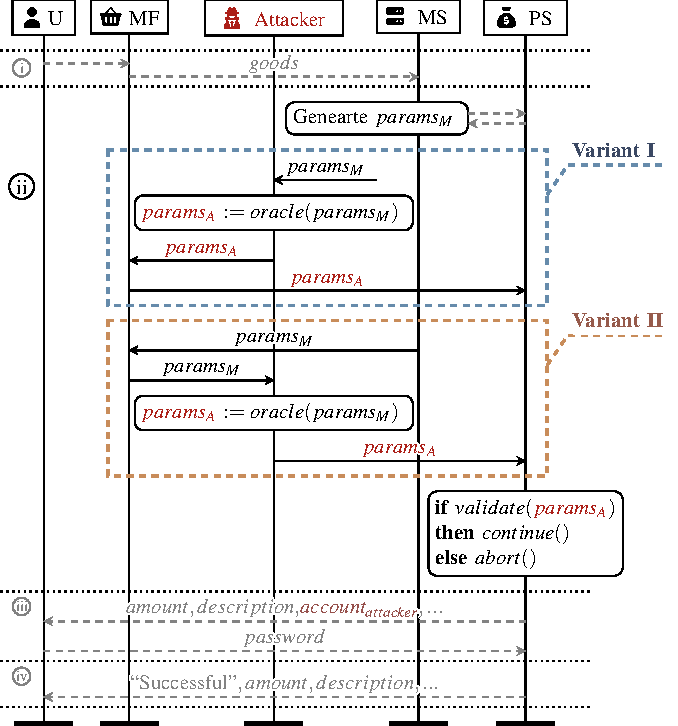
\includegraphics[width=\linewidth]{img/attack.pdf}
%DIFDELCMD <   %%%
\DIFdelendFL \DIFaddbeginFL 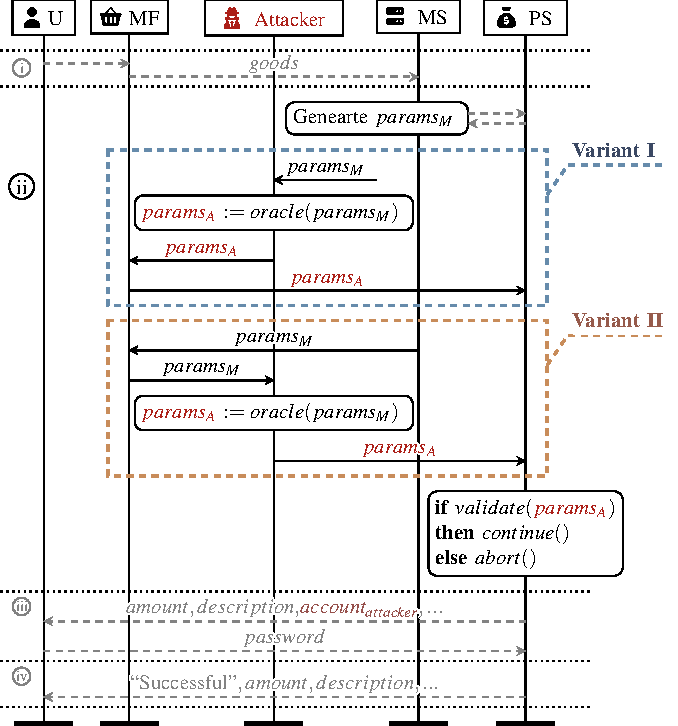
\includegraphics[width=0.85\linewidth]{img/attack.pdf}
  \DIFaddendFL \caption{
    Order Tampering Attack Variants. 
    Notation: 
      $params_M$ denotes the original payment parameters generated by the merchant;
      $params_A$ denotes the payment parameters after being tampered with by the adversary;
      $oracle(params_M)$ denotes the process by which the adversary generates payment parameters such that the order information remains fully consistent with $params_M$.
  }
  \label{fig:order_tampering_variants}
\end{figure}

The order tampering attack was first identified by \cite{Yang2017FlawedImplementations} in the in-app payment scenario.
Our formal analysis reveals that \emph{this attack is pervasive across all payment scenarios and all payment patterns}.
As long as any insecure channel exists, an adversary can successfully launch this attack.
Through an analysis of counterexamples violating IA-O1 and IA-O2, we identify two variants of the order tampering attack under different channel assumptions.
Figure~\ref{fig:order_tampering_variants} illustrates these two variants.
In Variant~\Rom{1}, the adversary targets the channel \emph{MF} $\Longleftrightarrow$ \emph{MS}, causing \emph{U} to ultimately authorize an attacker-specified order.
In Variant~\Rom{2}, the adversary tampers with the order on the channel \emph{MF} $\Longleftrightarrow$ \emph{PS}.

In prior work~\cite{Yang2017FlawedImplementations, Yang2019SecurityPayment, Lou2021PaymentVulnerabilities}, discussions of order tampering attacks primarily focus on Variant~\Rom{1}.
Under the channel assumptions of SecurePS, all counterexamples that violate the security properties originate from order tampering attacks on Variant~\Rom{1}.
However, our analysis under the channel assumptions of SecureMS indicates that Variant~\Rom{2} also has the potential to be successfully exploited in real-world settings.
In Section~\ref{sec:real_world}, we present a widely prevalent vulnerability that we discovered, which can be exploited to launch a Variant~\Rom{2} order tampering attack.


%-------------------------------------------------------------------------------
\section{Real-World Attacks} \label{sec:real_world}
%-------------------------------------------------------------------------------

In this section, we present a real-world attack \DIFdelbegin \DIFdel{case that was identified }\DIFdelend inspired by our analysis results\DIFdelbegin \DIFdel{and successfully carried out in practice.
We also introduce our measurement study to assess the scope and practical extent of the vulnerability's impactacross affected systems.
We further discuss the responsible vulnerability }\DIFdelend \DIFaddbegin \DIFadd{, a measurement study of its impact, and the responsible }\DIFaddend disclosure process.

\subsection{A Real-World Vulnerability}

Inspired by the Variant~\Rom{2} attack, we identified an exploitable vulnerability on the Android platform.
\DIFdelbegin \DIFdel{When initiating a payment request, merchant's Android applications use the Android Intent mechanism to }\DIFdelend \DIFaddbegin \DIFadd{Merchant applications }\DIFaddend transmit payment parameters to the \DIFdelbegin \DIFdel{payment service application.
As a core inter-component communication mechanism provided by the Android system, Intent serves as the primary means by which the }\DIFdelend PSP-B and Alipay \DIFdelbegin \DIFdel{receive payment parameters from merchant applications .
A merchant application typically constructs an Intent containing payment parameters and uses it to launch the corresponding payment application.
}%DIFDELCMD < 

%DIFDELCMD < %%%
\DIFdel{It should be noted that Intents can be classified into two categories, explicit Intents and implicit Intents. 
}\DIFdelend \DIFaddbegin \DIFadd{applications through the Android Intent mechanism.
}\DIFaddend An explicit Intent specifies the fully qualified package name of the target application, whereas an implicit Intent only declares the action, category, and data, \DIFdelbegin \DIFdel{allowing the system to match and select }\DIFdelend \DIFaddbegin \DIFadd{and the system selects }\DIFaddend a responding component based on Intent Filters.
\DIFdelbegin \DIFdel{The security risk primarily arises from the misuse of implicit Intents.
}%DIFDELCMD < 

%DIFDELCMD < %%%
\DIFdel{When requesting a payment, a }\DIFdelend \DIFaddbegin \DIFadd{A }\DIFaddend merchant application should \DIFaddbegin \DIFadd{therefore }\DIFaddend use an explicit Intent to \DIFdelbegin \DIFdel{explicitly designate the PSP-B or Alipay applications as the target, thereby ensuring }\DIFdelend \DIFaddbegin \DIFadd{ensure }\DIFaddend that the payment request is \DIFdelbegin \DIFdel{correctly routed to a }\DIFdelend \DIFaddbegin \DIFadd{routed to the }\DIFaddend trusted payment application.
However, we find that some merchant applications use implicit Intents in practice\DIFdelbegin \DIFdel{.
This means that }\DIFdelend \DIFaddbegin \DIFadd{, so }\DIFaddend an attacker can hijack payment requests \DIFdelbegin \DIFdel{originally sent to a payment application }\DIFdelend by deploying a malicious application that declares the same Intent handling capability.
\DIFdelbegin %DIFDELCMD < 

%DIFDELCMD < %%%
\DIFdelend Intent hijacking is \DIFdelbegin \DIFdel{not specific to payment scenarios, but rather a systemic security risk inherent in the }\DIFdelend \DIFaddbegin \DIFadd{a systemic risk of }\DIFaddend Android component communication\DIFdelbegin \DIFdel{mechanism.
However, }\DIFdelend \DIFaddbegin \DIFadd{, yet }\DIFaddend existing third-party online payment protocols are designed under the assumption that the \DIFdelbegin \DIFdel{communication }\DIFdelend channel between the merchant client and the payment application is trusted.
\DIFdelbegin \DIFdel{This channel assumption is unrealistic in real-world deployments.
}\DIFdelend 

\subsection{Attack Implementation}

\DIFdelbegin %DIFDELCMD < \begin{figure}[t]
%DIFDELCMD <   \centering
%DIFDELCMD <   %%%
%DIF <  --- 左侧子图：受害者设备 ---
  %DIFDELCMD < \begin{subfigure}[b]{0.32\linewidth}
%DIFDELCMD <     \centering
%DIFDELCMD <     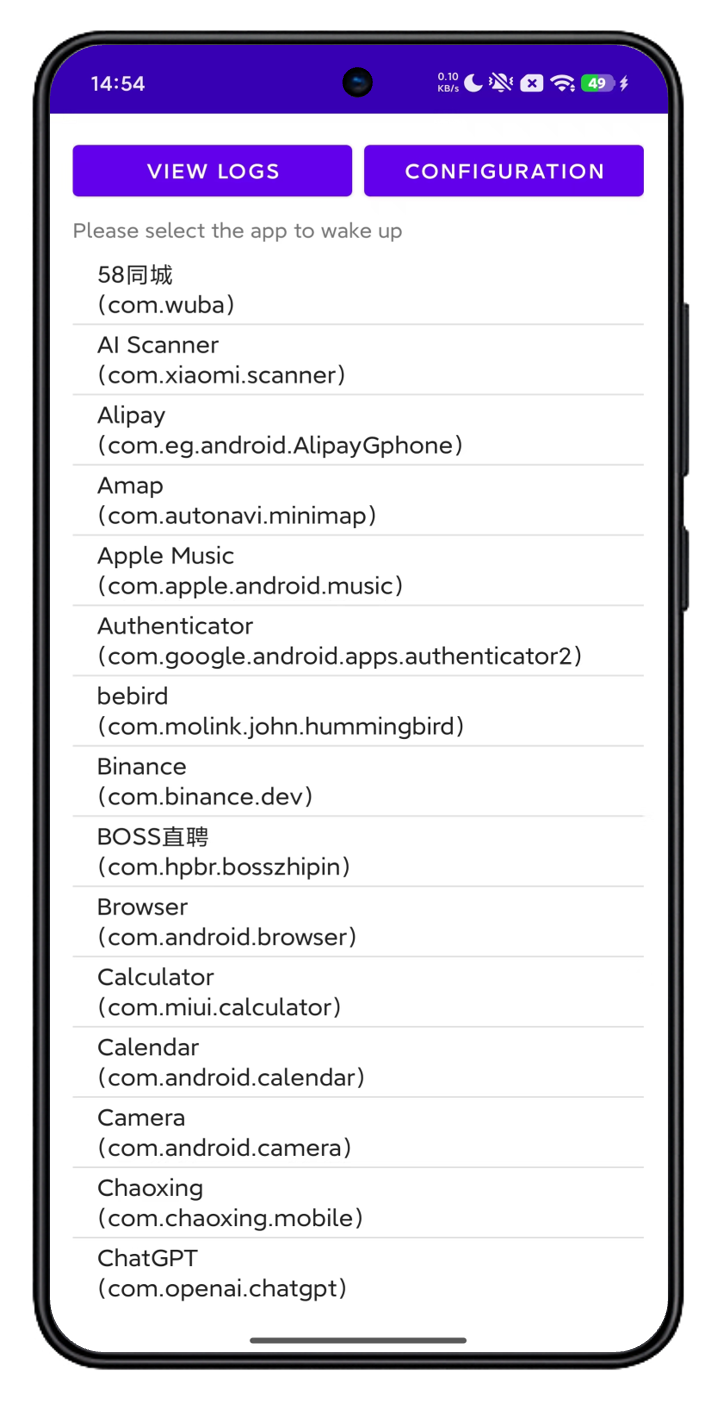
\includegraphics[width=\linewidth]{img/setup_1.png} %%%
%DIF <  请替换为受害者设备的图片路径
    %DIFDELCMD < \caption{%
{%DIFAUXCMD
\DIFdelFL{Victim Device}}
    %DIFAUXCMD
%DIFDELCMD < \label{fig:victim_device}
%DIFDELCMD <   \end{subfigure}
%DIFDELCMD <   %%%
\DIFdelFL{\hspace{3em}
  %DIF <  --- 右侧子图：攻击者设备 ---
  }%DIFDELCMD < \begin{subfigure}[b]{0.32\linewidth}
%DIFDELCMD <     \centering
%DIFDELCMD <     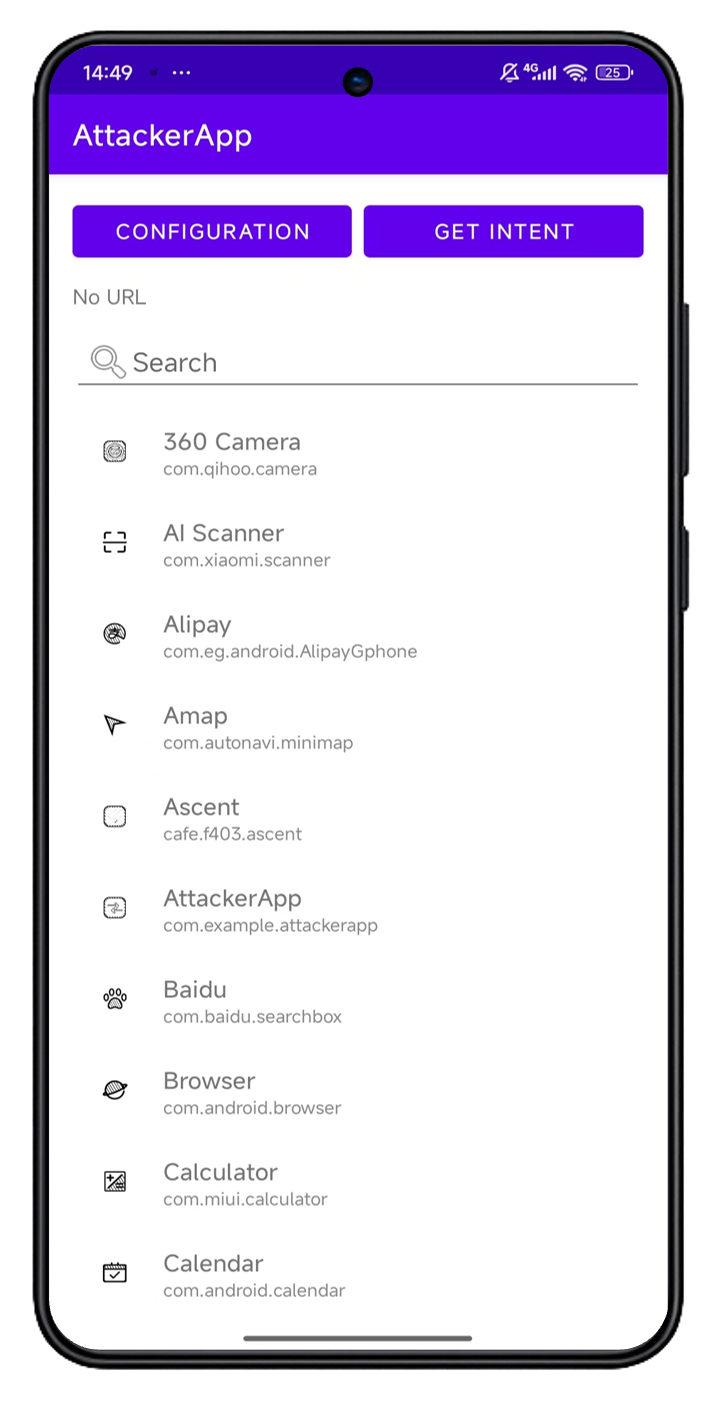
\includegraphics[width=\linewidth]{img/setup_2.png} %%%
%DIF <  请替换为攻击者设备的图片路径
    %DIFDELCMD < \caption{%
{%DIFAUXCMD
\DIFdelFL{Attacker Device}}
    %DIFAUXCMD
%DIFDELCMD < \label{fig:attacker_device}
%DIFDELCMD <   \end{subfigure}
%DIFDELCMD < 

%DIFDELCMD <   %%%
%DIFDELCMD < \caption{%
{%DIFAUXCMD
\DIFdelFL{Attack Setup. 
    Device~\ref{fig:victim_device} denotes the victim device, which installs the malicious application, a vulnerable merchant application, and a payment application. 
    Device~\ref{fig:attacker_device} denotes the attacker device, which installs the attacker application. 
    The screenshots correspond to the real interfaces of the malicious and attacker applications, respectively.
  }}
  %DIFAUXCMD
%DIFDELCMD < \label{fig:real_world_attack_devices}
%DIFDELCMD < \end{figure}
%DIFDELCMD < 

%DIFDELCMD < %%%
\DIFdelend We developed two Android applications, a malicious application and an attacker application, to exploit the aforementioned vulnerability.
\DIFdelbegin \DIFdel{Fig.~\ref{fig:real_world_attack_devices} illustrates the devices used in the attack, serving as the victim device and the attacker device, respectively, with the corresponding applications installed.
The malicious application on device~\ref{fig:victim_device} }\DIFdelend \DIFaddbegin \DIFadd{The victim device runs the malicious application, a vulnerable merchant application, and a payment application; the malicious application }\DIFaddend is responsible for capturing and replaying payment parameters.
The attacker \DIFdelbegin \DIFdel{application on device ~\ref{fig:attacker_device} }\DIFdelend \DIFaddbegin \DIFadd{device runs the attacker application, which }\DIFaddend places orders on the merchant platform and returns payment parameters to the malicious application.

Fig.~\ref{fig:real_world_attack_flow} illustrates the workflow of the new order tampering attack\DIFdelbegin \DIFdel{.
The attack }\DIFdelend \DIFaddbegin \DIFadd{, which }\DIFaddend proceeds in four phases\DIFdelbegin \DIFdel{:
}%DIFDELCMD < \begin{enumerate}[leftmargin=*]
%DIFDELCMD <   \item %%%
\DIFdelend \DIFaddbegin \DIFadd{.
(1)~}\DIFaddend A benign merchant application \DIFdelbegin \DIFdel{initiates a payment request by dispatching }\DIFdelend \DIFaddbegin \DIFadd{dispatches }\DIFaddend an implicit Intent containing payment parameters to the payment application\DIFdelbegin \DIFdel{;
  }%DIFDELCMD < \item %%%
\DIFdelend \DIFaddbegin \DIFadd{.
(2)~}\DIFaddend By hijacking the Intent resolution process, the malicious application intercepts the original payment parameters and extracts the embedded order information\DIFdelbegin \DIFdel{;
  }%DIFDELCMD < \item %%%
\DIFdelend \DIFaddbegin \DIFadd{.
(3)~}\DIFaddend Using the extracted information, the attacker application places a new order under an attacker-controlled account on the merchant platform and obtains \DIFdelbegin \DIFdel{a fresh set of }\DIFdelend \DIFaddbegin \DIFadd{fresh }\DIFaddend payment parameters that preserve the original order information while being bound to the attacker's account\DIFdelbegin \DIFdel{;
  }%DIFDELCMD < \item %%%
\DIFdelend \DIFaddbegin \DIFadd{.
(4)~}\DIFaddend The tampered payment parameters are \DIFdelbegin \DIFdel{then }\DIFdelend relayed to the payment application, which processes the request without detecting the modification.
\DIFdelbegin %DIFDELCMD < \end{enumerate}
%DIFDELCMD < %%%
\DIFdelend As a result, the attacker successfully tampers with the order, causing the user to complete a payment specified by the attacker rather than the original merchant.

\begin{figure}[t]
  \centering
  \DIFdelbeginFL %DIFDELCMD < 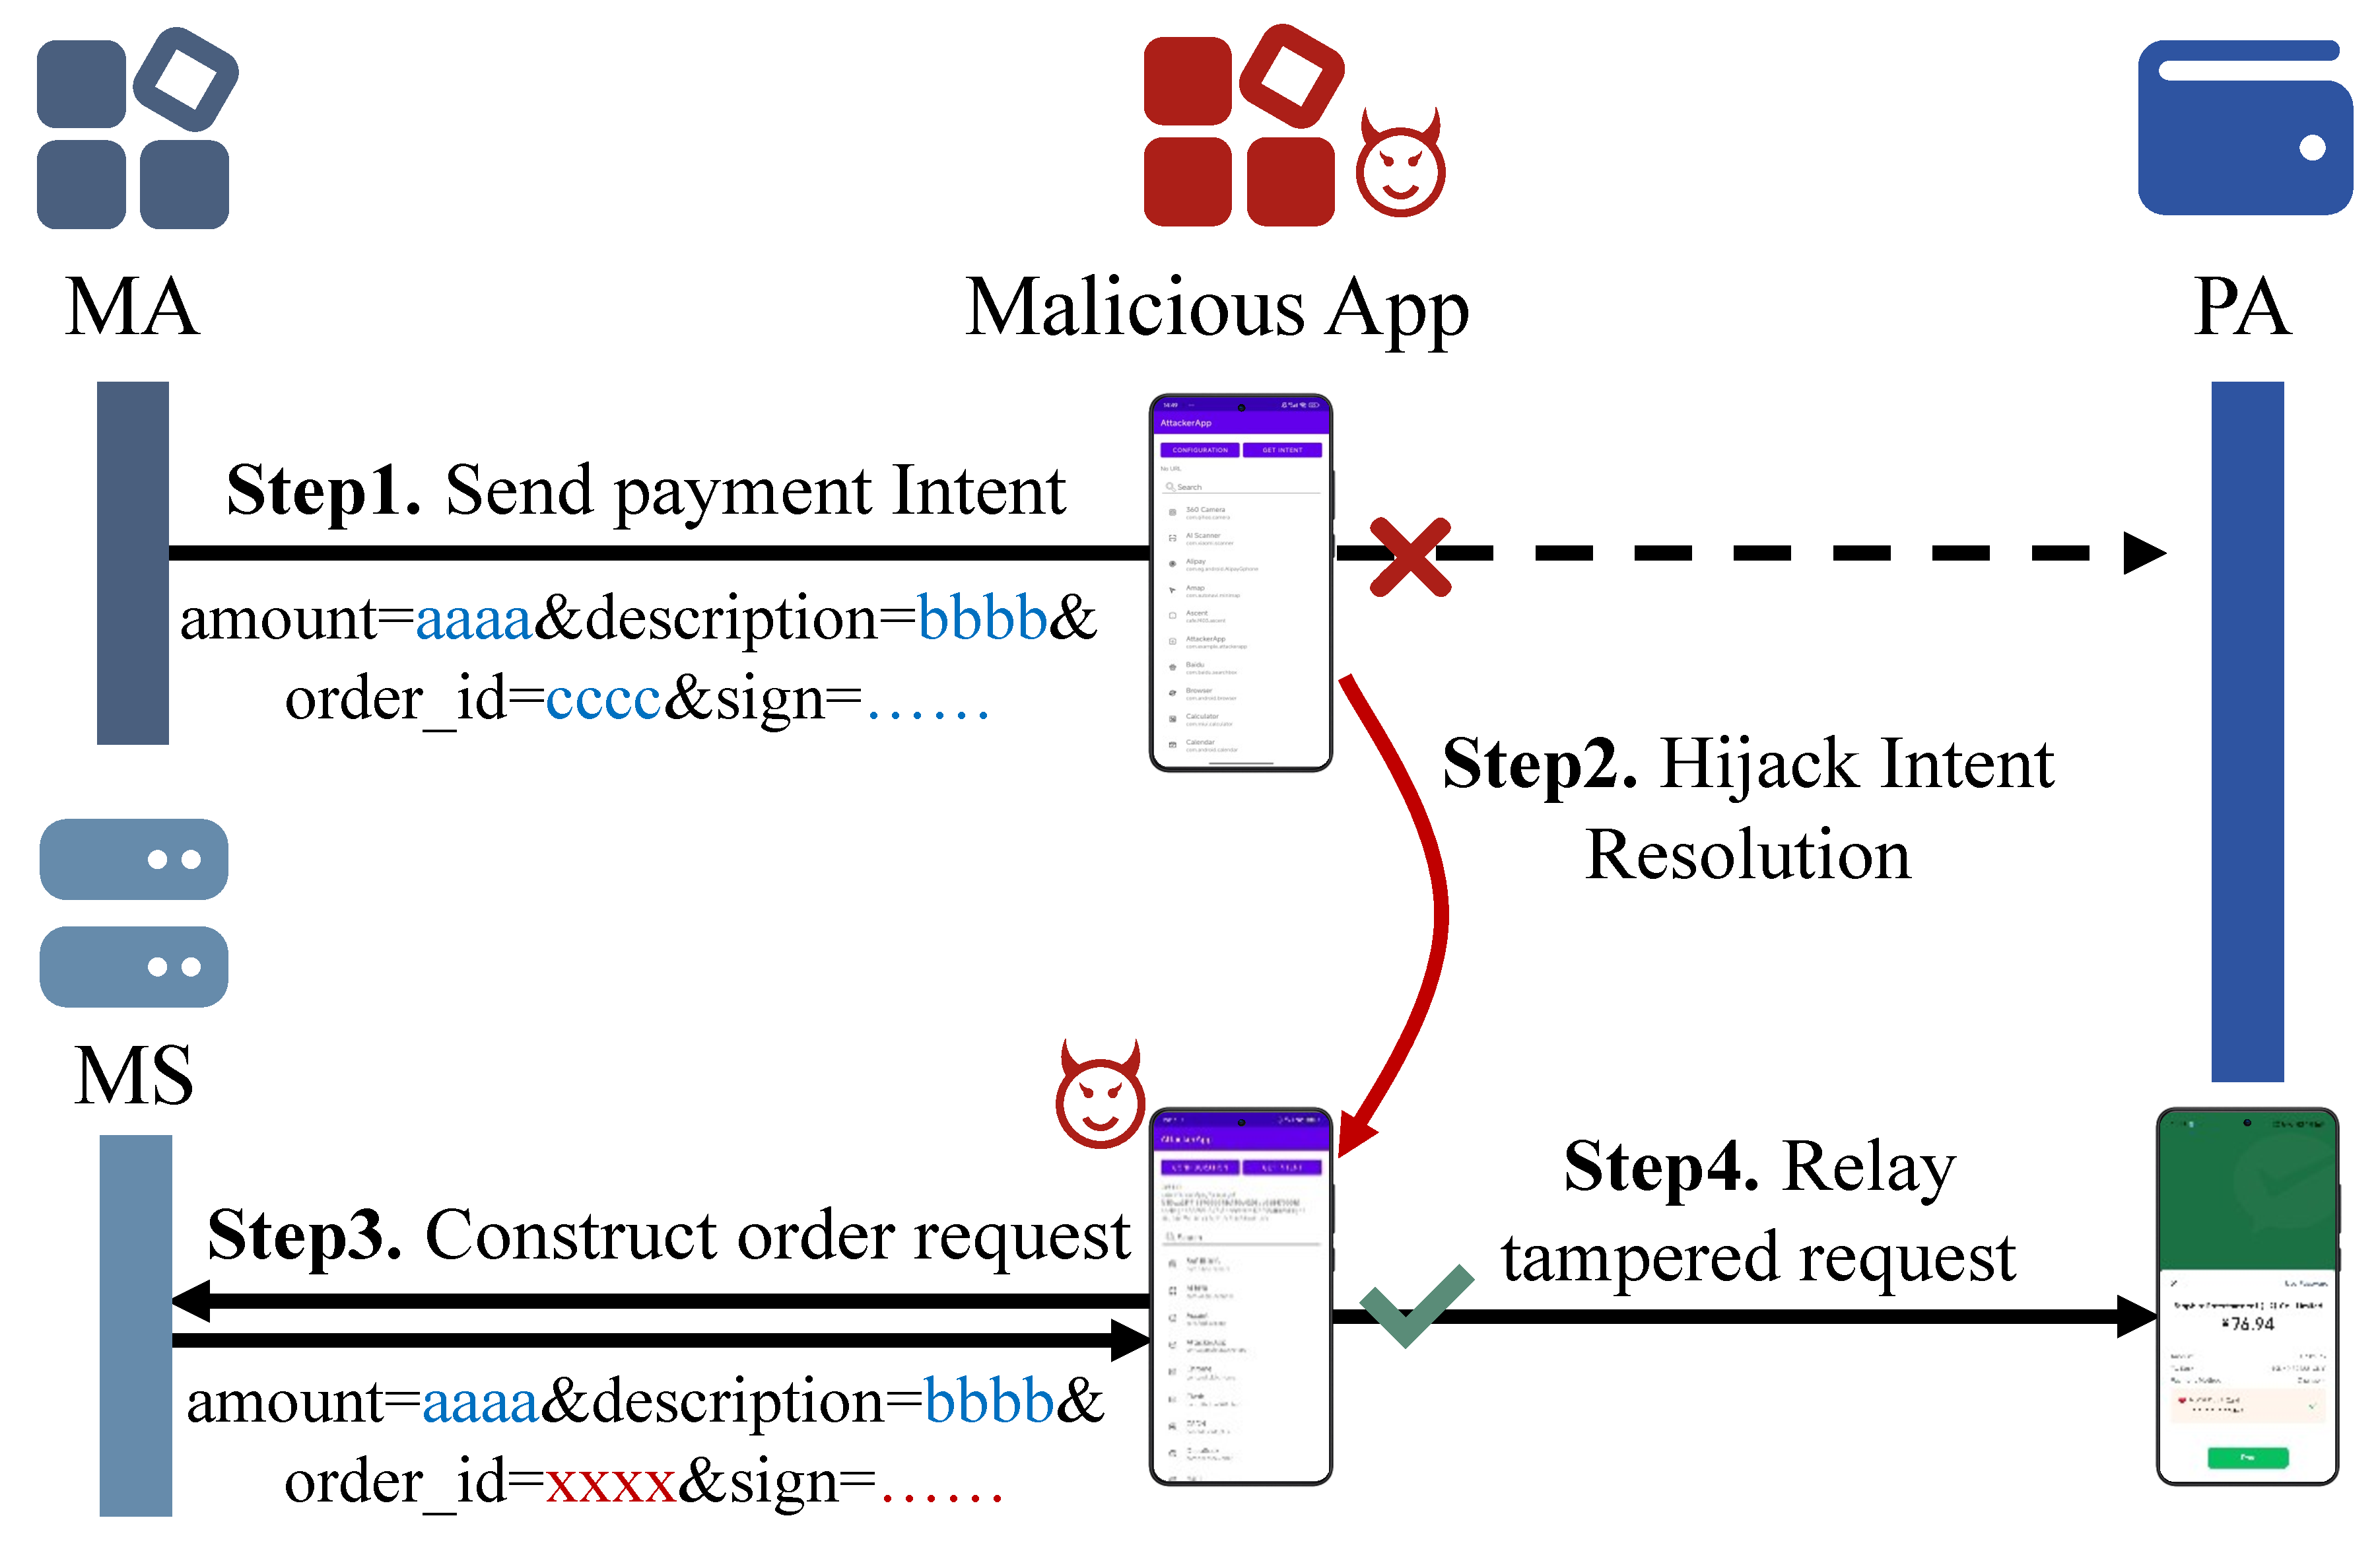
\includegraphics[width=\linewidth]{img/attack_flow.pdf}
%DIFDELCMD <   %%%
\DIFdelendFL \DIFaddbeginFL 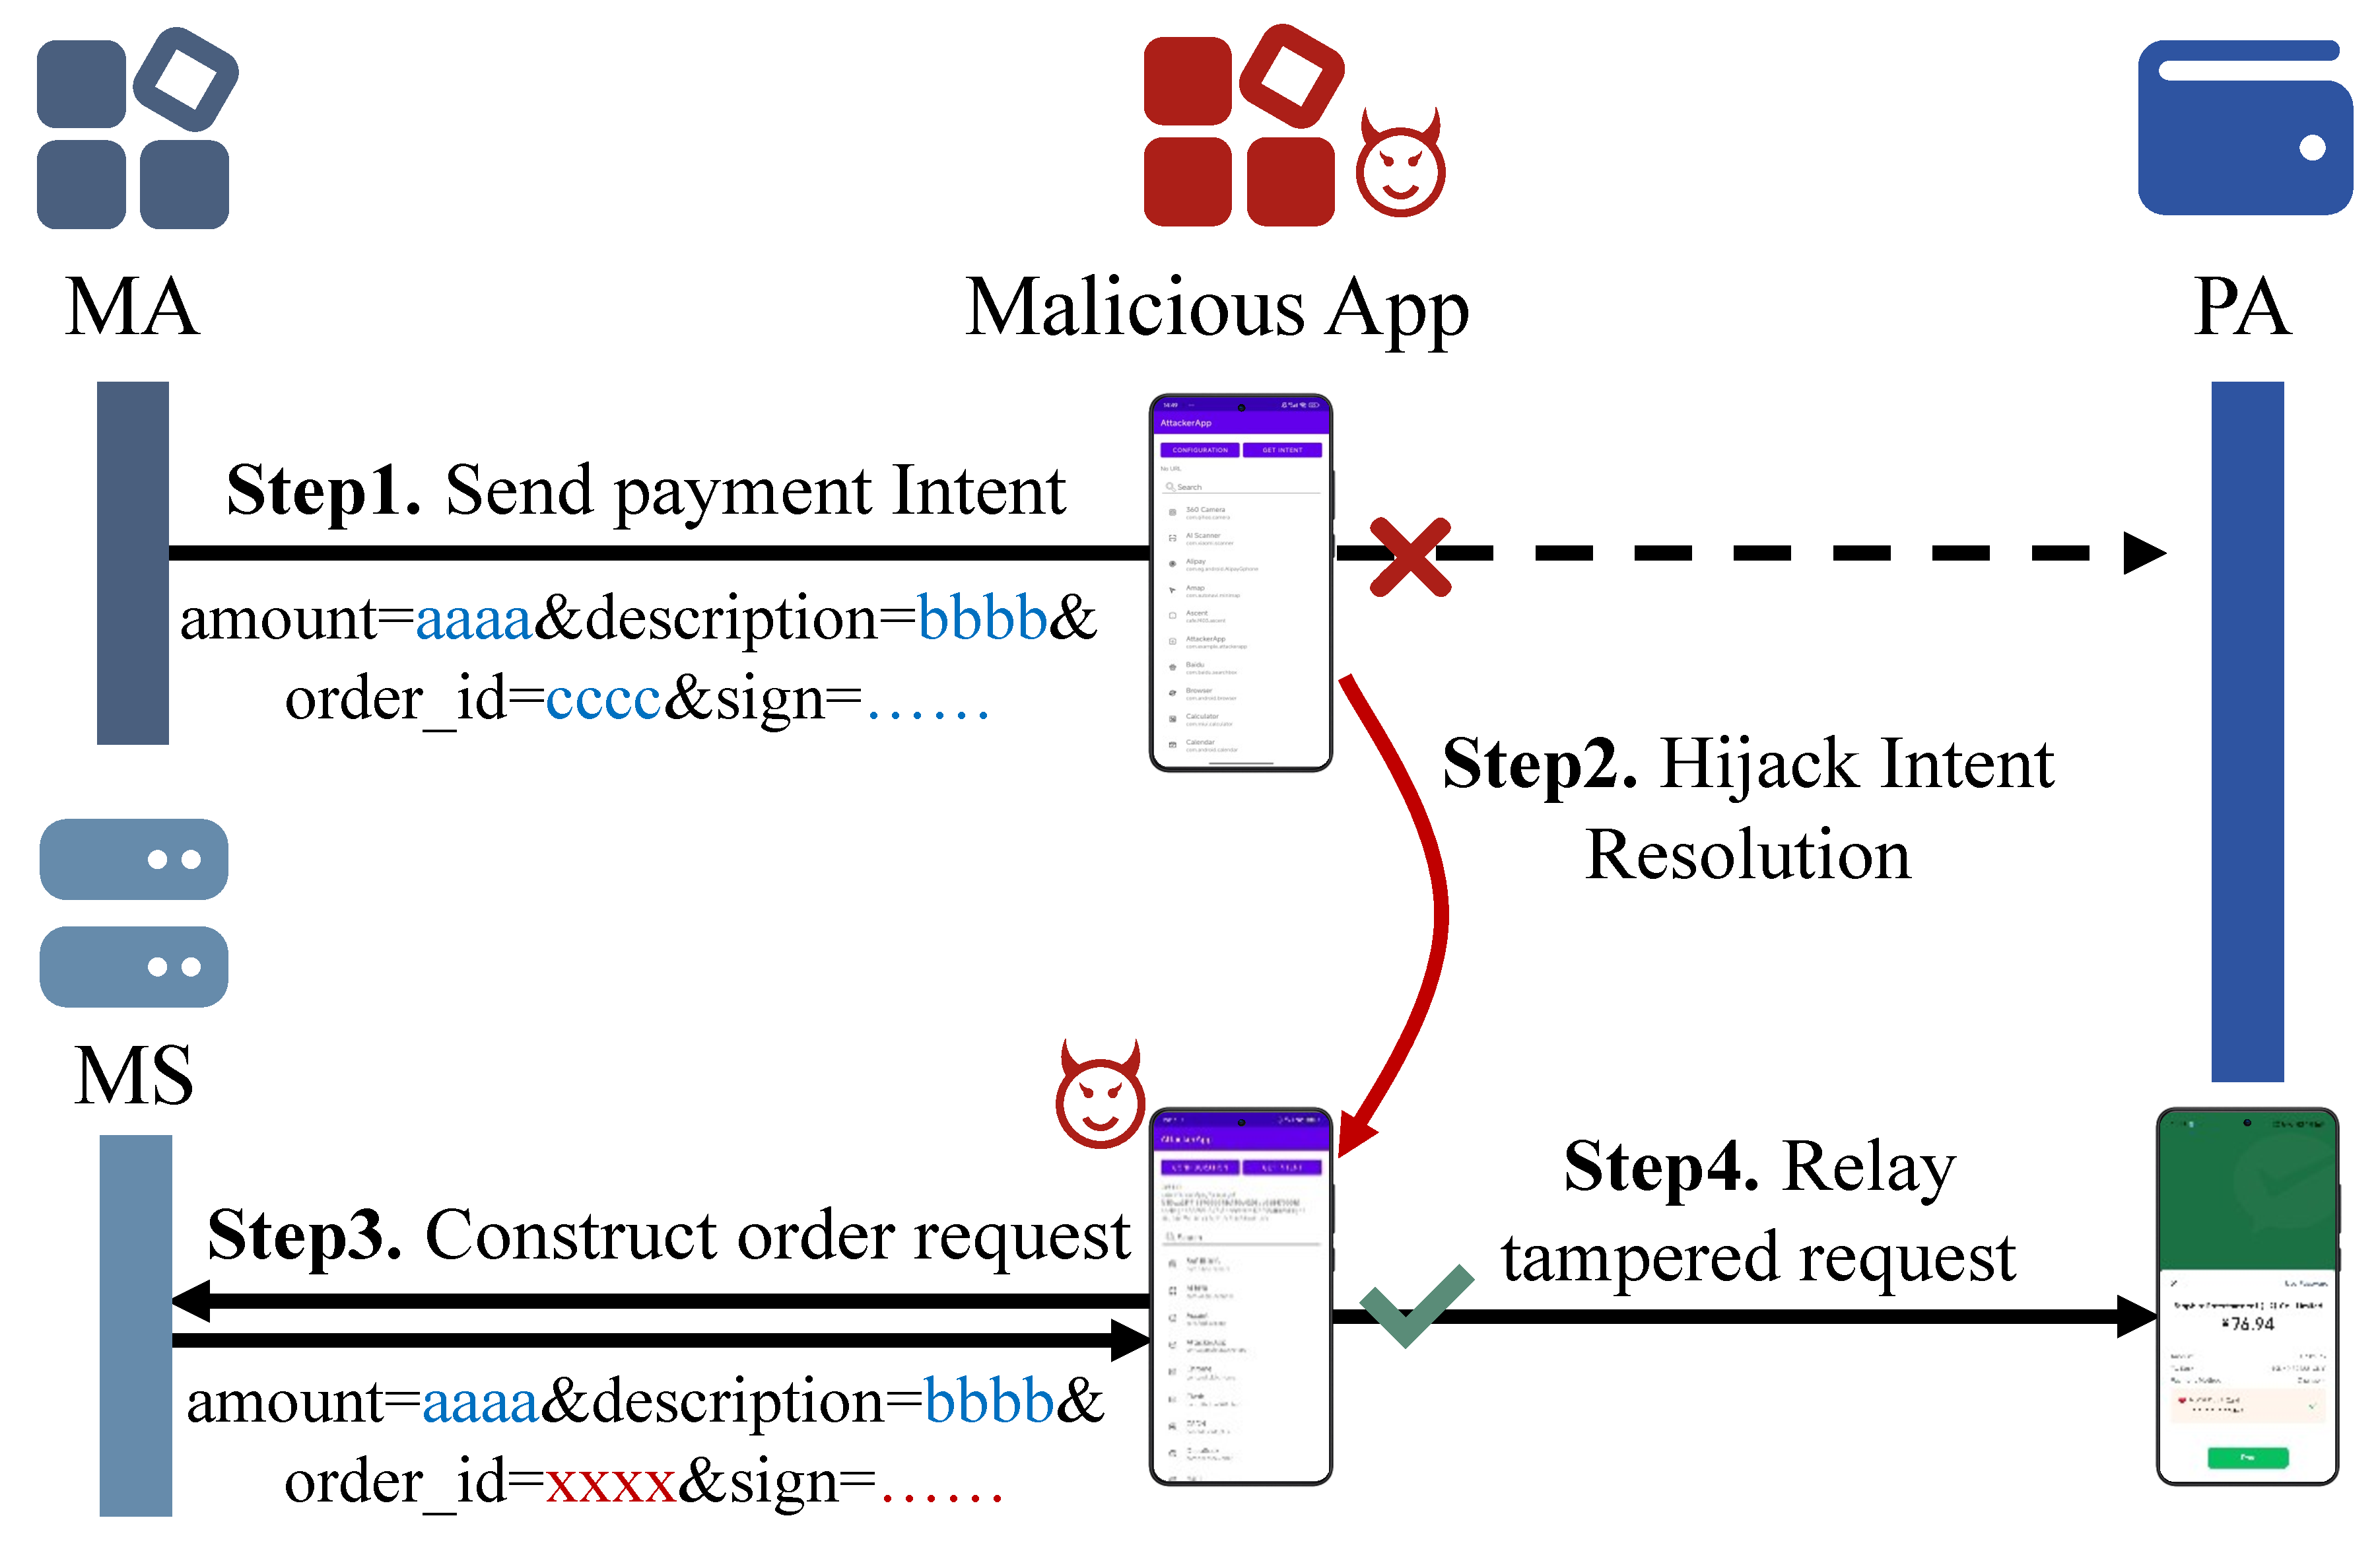
\includegraphics[width=0.85\linewidth]{img/attack_flow.pdf}
  \DIFaddendFL \caption{Attack Flow.
    MA denotes the merchant application; 
    Malicious Application denotes the malicious application we developed;
    PA denotes the payment application;
    MS denotes the merchant server.
  }
  \label{fig:real_world_attack_flow}
\end{figure}

\subsection{Impact Assessment}
To assess the real-world impact of the identified vulnerability, we conducted a manual measurement study on Android applications and games that integrate the PSP-B or Alipay SDK.
Our dataset consists of 150 popular Android applications and 50 games, covering up to the three most recent versions of each application and the latest version of each game.
For some applications, only one or two versions were available\DIFdelbegin \DIFdel{.
In total, we collected }\DIFdelend \DIFaddbegin \DIFadd{, giving }\DIFaddend 461 application versions \DIFaddbegin \DIFadd{in total}\DIFaddend .

Among these versions, 419 support PSP-B and 401 support Alipay.
Our analysis reveals that 64 PSP-B–enabled versions and 72 Alipay-enabled versions are vulnerable.
Out of 53 applications, a total of 116 versions representing more than 25\% of the analyzed dataset support at least one vulnerable payment method. 
These vulnerable applications span a wide range of categories, including e-commerce, online education, and entertainment.
Their cumulative download count reaches 265.85 billion, indicating that the vulnerability potentially affects a very large user base and poses a significant security risk in practice.

\subsection{Responsible Disclosure}
Following responsible disclosure guidelines, we reported the vulnerability to the security teams of PSP-B and Alipay in December 2025. 
At the time of writing, both providers had acknowledged the issue and confirmed that remediation efforts were underway. 
We identified contact information for 41 affected Android applications and issued security notifications to their developers, detailing the underlying risks and corresponding mitigation strategies.
Among these, 17 developers responded; one explicitly committed to fixing the vulnerability, while the remaining vendors attributed the issue to the Alipay and PSP-B SDKs.
We did not notify the Google Play Store, as Chinese apps are distributed mainly through vendor stores and the root cause lies in the Alipay and PSP-B SDKs, which a single update can fix for all integrating apps. Other major systems (Apple Pay, Stripe, etc.) use architectures not exposed to this attack.
\DIFaddbegin 

\DIFaddend %-------------------------------------------------------------------------------
\section{Countermeasure} \DIFaddbegin \label{sec:countermeasure}
\DIFaddend %-------------------------------------------------------------------------------
% In this section, we xxxx.

In this section, we analyze the causes of order tampering attacks\DIFdelbegin \DIFdel{and }\DIFdelend \DIFaddbegin \DIFadd{, }\DIFaddend introduce our countermeasure\DIFdelbegin \DIFdel{.
%DIF <  Then, we present the symbolic verification results of our countermeasure and discuss its advantages and limitations.
Then, we verify our countermeasure }\DIFdelend \DIFaddbegin \DIFadd{, verify it }\DIFaddend using symbolic methods\DIFdelbegin \DIFdel{and present the results.
Finally, we discuss our countermeasure}\DIFdelend \DIFaddbegin \DIFadd{, and discuss it}\DIFaddend .

\subsection{Cause Analysis}

\textbf{Superficial Causes.}
From a superficial perspective, order tampering attacks arise from \DIFdelbegin \DIFdel{the existence of }\DIFdelend insecure communication channels between \emph{MS} and \emph{PS-App}\DIFdelbegin \DIFdel{.
An attacker can intercept and }\DIFdelend \DIFaddbegin \DIFadd{, over which an attacker can }\DIFaddend tamper with order information \DIFdelbegin \DIFdel{along this channel, thereby misleading }\DIFdelend \DIFaddbegin \DIFadd{and mislead }\DIFaddend the user into authorizing an incorrect payment.
\DIFdelbegin \DIFdel{At first glance, addressing this issue appears straightforward.
It suffices to ensure that the communication channels between }\emph{\DIFdel{MS}} %DIFAUXCMD
\DIFdel{and }\emph{\DIFdel{PS-App}} %DIFAUXCMD
\DIFdel{are secure.
However, }\DIFdelend \DIFaddbegin \DIFadd{Securing these channels is difficult }\DIFaddend for payment service providers \DIFdelbegin \DIFdel{, this seemingly simple solution is difficult to realize in practice.
The security of the communication }\DIFdelend \DIFaddbegin \DIFadd{in practice: the }\DIFaddend path from merchant backends to \emph{PS-App} \DIFdelbegin \DIFdel{is influenced by both merchants and end users, and is largely beyond the control of payment service providers.
Payment service providers serve }\DIFdelend \DIFaddbegin \DIFadd{depends on the backend implementations of }\DIFaddend a large number of merchants \DIFdelbegin \DIFdel{, each with diverse backend implementations, making it infeasible to ensure that all merchants correctly secure their communication channels.
Similarly, merchants serve }\DIFdelend \DIFaddbegin \DIFadd{and on the network environments of }\DIFaddend a vast user base\DIFdelbegin \DIFdel{with heterogeneous device environments, and payment service providerscannot guarantee that all users operate within secure network conditions.
Therefore, defending against order tampering attacks solely by securing communication channels is, in practice, highly challenging.
}\DIFdelend \DIFaddbegin \DIFadd{, both of which lie beyond the providers' control.
}\DIFaddend Consequently, mitigation is often reactive: once an insecure communication channel is identified, merchants and users are notified to apply patches.

\textbf{Root Causes.}
The root cause of such attacks lies in the lack of a user-side authentication mechanism for order information in existing payment patterns.
\DIFdelbegin \DIFdel{We examine the typical actions performed by users during the paymentprocess: entering }\DIFdelend \DIFaddbegin \DIFadd{During payment, the user enters }\DIFaddend a payment password to authorize the transaction \DIFdelbegin \DIFdel{, and possibly verifying }\DIFdelend \DIFaddbegin \DIFadd{and possibly checks }\DIFaddend the payment amount and description.
\DIFdelbegin \DIFdel{However, the user does not actually authenticate the order.
Information such as the payment amount and item description merely represents the }\DIFdelend \DIFaddbegin \DIFadd{These values describe the }\DIFaddend content of the current payment, \DIFdelbegin \DIFdel{and does not correspond to }\DIFdelend \DIFaddbegin \DIFadd{not }\DIFaddend the original order that the user intends to confirm\DIFdelbegin \DIFdel{.
In other words, during the }\emph{\DIFdel{Authentication}} %DIFAUXCMD
\DIFdel{phase, the userperforms no form of authentication of the order data.
The user}\DIFdelend \DIFaddbegin \DIFadd{, so the user}\DIFaddend 's authorization \DIFdelbegin \DIFdel{is applied }\DIFdelend \DIFaddbegin \DIFadd{applies }\DIFaddend only to the act of payment \DIFdelbegin \DIFdel{transaction, }\DIFdelend rather than to a specific order.
Once an attacker is able to tamper with order parameters in transit, the user can be induced to authorize an incorrect order.
\DIFdelbegin \DIFdel{This observation reveals a design flaw in current payment patterns}\DIFdelend \DIFaddbegin 

\DIFadd{An order created through the order oracle carries the same amount, description, and payee as the user's order, so it passes every check the user performs; the two orders differ only in the order instance and in the account that placed it.
}\emph{\DIFadd{PS}} \DIFadd{cannot tell them apart either, because it cannot authenticate the sender of the payment parameters, so a countermeasure has to give }\emph{\DIFadd{PS}} \DIFadd{a check, carried by the user, that the attacker cannot reproduce with its own order}\DIFaddend .

\subsection{\DIFdelbegin \DIFdel{Countermeasure }\DIFdelend Design \DIFaddbegin \DIFadd{Goals}\DIFaddend }

\DIFdelbegin %DIFDELCMD < \begin{figure}[t]
%DIFDELCMD <   \centering
%DIFDELCMD <   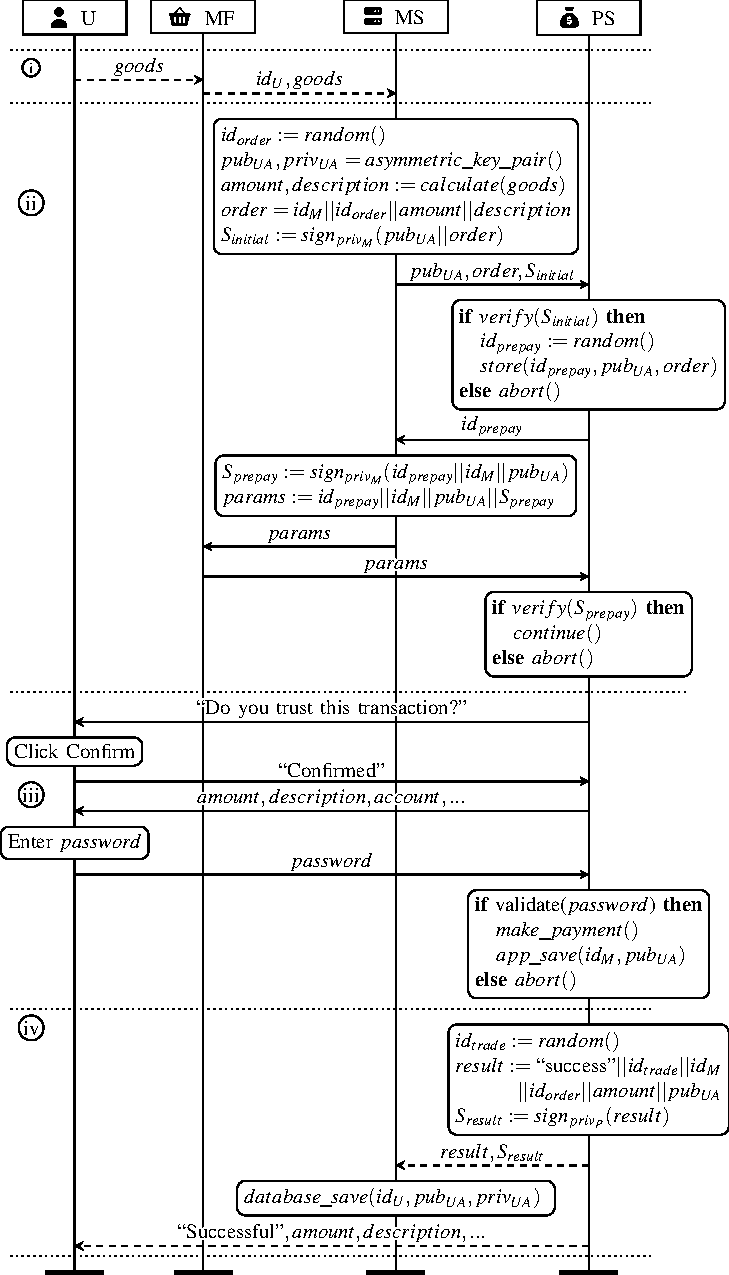
\includegraphics[width=\linewidth]{img/cm_initial.pdf}
%DIFDELCMD <   %%%
%DIFDELCMD < \caption{%
{%DIFAUXCMD
\DIFdelFL{Initial Payment}}
  %DIFAUXCMD
%DIFDELCMD < \label{fig:our_model_initial}
%DIFDELCMD < \end{figure}
%DIFDELCMD < %%%
\DIFdelend \DIFaddbegin \DIFadd{A countermeasure against order tampering should meet three goals.
}\begin{enumerate}[leftmargin=*, label=\textbf{G\arabic*}]
  \item \textbf{\DIFadd{Security under weak channel assumptions.}} \DIFadd{The protocol satisfies all security properties of Section~\ref{sec:security_properties} when both }\emph{\DIFadd{MF}} \DIFadd{$\Longleftrightarrow$ }\emph{\DIFadd{MS}} \DIFadd{and }\emph{\DIFadd{MF}} \DIFadd{$\Longleftrightarrow$ }\emph{\DIFadd{PS}} \DIFadd{are insecure, without requiring the user to recognize the payee account.
  }\item \textbf{\DIFadd{No per-user state.}} \DIFadd{Each payment completes in one protocol run without long-term keys or bindings for individual users, so the first payment to a merchant is protected like any other.
  }\item \textbf{\DIFadd{Small changes for merchants.}} \DIFadd{Merchants keep the existing message flow and notification interface; the signed order gains one field, the user account.
}\end{enumerate}
\DIFadd{Our countermeasure, Sealed Checkout Code (SCC), meets all three goals.
}\DIFaddend 

\DIFaddbegin \subsection{\DIFadd{Countermeasure Design}}

\DIFaddend \begin{figure}[t]
  \centering
  \DIFdelbeginFL %DIFDELCMD < 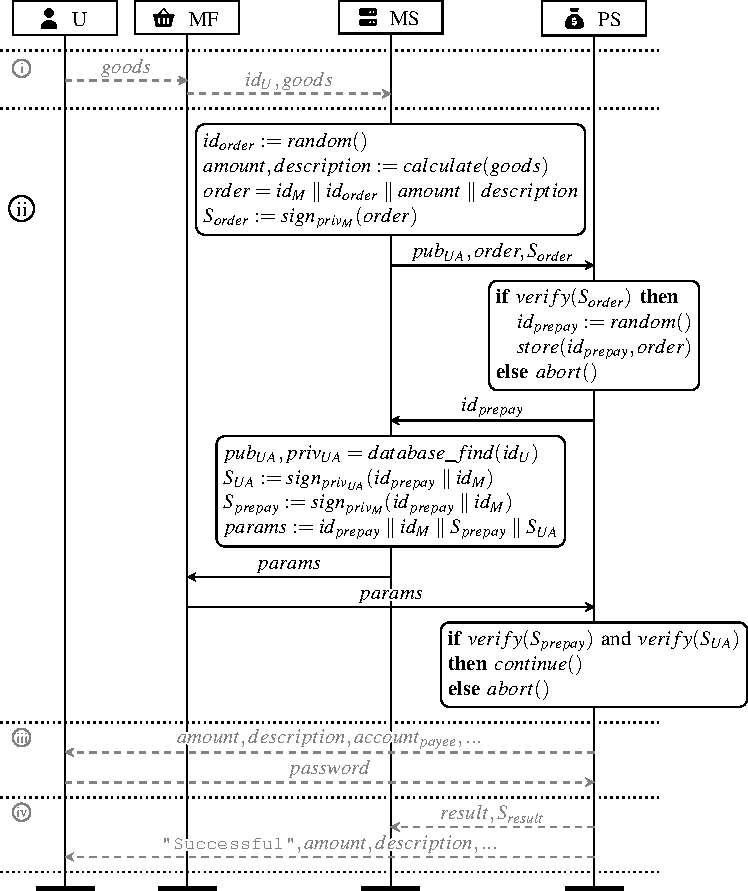
\includegraphics[width=\linewidth]{img/cm_regular.pdf}
%DIFDELCMD <   %%%
%DIFDELCMD < \caption{%
{%DIFAUXCMD
\DIFdelFL{Regular Payment}}
  %DIFAUXCMD
%DIFDELCMD < \label{fig:our_model_regular}
%DIFDELCMD < %%%
\DIFdelendFL \DIFaddbeginFL 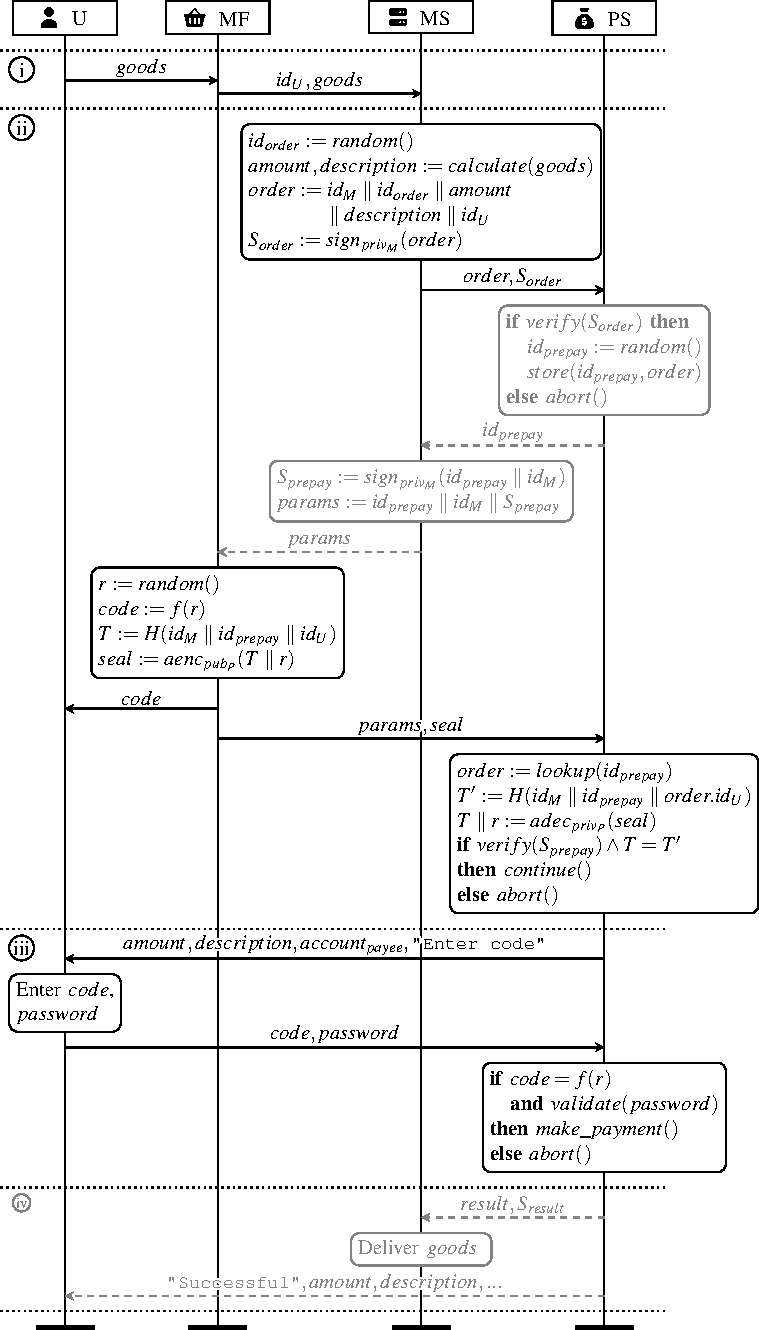
\includegraphics[width=0.85\linewidth]{img/cm_scc.pdf}
  \caption{\DIFaddFL{Sealed Checkout Code on top of payment pattern~B.
    Black elements are new or changed; gray elements are identical to pattern~B.
    Notation: $id_{U}$ denotes the user's account at the merchant; $H$ denotes a hash function; $aenc_{k}(m)$ and $adec_{k}(c)$ denote public-key encryption and decryption; $f$ maps a nonce to a short code; $lookup(id_{prepay})$ returns the order that }\emph{\DIFaddFL{PS}} \DIFaddFL{recorded for $id_{prepay}$.}}
  \label{fig:cm_scc}
\DIFaddendFL \end{figure}

\DIFdelbegin \DIFdel{To fundamentally address order tampering attacks, we design and propose a new third-party payment protocol that introduces a user-side order authentication mechanism to effectively prevent such attacks.
  Our payment protocol distinguishes between }\emph{\DIFdel{initial}} %DIFAUXCMD
\DIFdelend \DIFaddbegin \DIFadd{SCC uses the user as the link between }\emph{\DIFadd{MF}} \DIFaddend and \DIFdelbegin \emph{\DIFdel{regular}} %DIFAUXCMD
\DIFdel{payments, whose workflows are illustrated in Fig.
  ~\ref{fig:our_model_initial} and Fig.
~\ref{fig:our_model_regular}, respectively.
For a given merchant and user, the first payment initiated by the user is defined as an }\emph{\DIFdel{initial}} %DIFAUXCMD
\DIFdel{payment , while all later payments are defined as }\emph{\DIFdel{regular}} %DIFAUXCMD
\DIFdel{payments}\DIFdelend \DIFaddbegin \emph{\DIFadd{PS}} \DIFadd{that the attacker does not control.
For each payment, }\emph{\DIFadd{MF}} \DIFadd{draws a fresh nonce $r$, seals it to }\emph{\DIFadd{PS}} \DIFadd{together with a digest of the order handle and the user's account, and shows a short code derived from $r$ to the user.
}\emph{\DIFadd{PS}} \DIFadd{accepts the seal only for the order it was created for, and completes the payment only if the user enters the same code.
Fig.~\ref{fig:cm_scc} shows the workflow on top of payment pattern~B}\DIFaddend .

\DIFdelbegin \DIFdel{At the beginning of the }\emph{\DIFdel{Prepayment}} %DIFAUXCMD
\DIFdel{phase of a }\DIFdelend \DIFaddbegin \textbf{\DIFadd{User account.}}
\DIFadd{$id_{U}$ denotes the account under which the user is logged in at the merchant.
}\emph{\DIFadd{MF}} \DIFadd{knows $id_{U}$ from the user's login, and }\emph{\DIFadd{MS}} \DIFadd{associates each order with the account of the logged-in user.
As in the rest of the paper, the }\DIFaddend user's \DIFdelbegin \DIFdel{initial payment, }\DIFdelend \DIFaddbegin \DIFadd{login session with }\DIFaddend \emph{MS} \DIFdelbegin \DIFdel{generates a public–private key pair $(priv_{UA}, pub_{UA})$ for }\emph{\DIFdel{U}}%DIFAUXCMD
\DIFdel{, and then uses the merchant private key $priv_M$ to sign $pub_{UA}$ together with the order information before sending them }\DIFdelend \DIFaddbegin \DIFadd{is authentic, and the attacker controls the payment messages on the two external channels.
An attacker places orders on accounts it controls, so every order created through the order oracle carries an account other than $id_{U}$.
}

\textbf{\DIFadd{Order Phase.}}
\DIFadd{The user selects $goods$ in }\emph{\DIFadd{MF}}\DIFadd{, and }\emph{\DIFadd{MF}} \DIFadd{sends $goods$ to }\emph{\DIFadd{MS}} \DIFadd{within the user's login session, which identifies $id_{U}$.
}

\textbf{\DIFadd{Prepayment Phase.}}
\emph{\DIFadd{MS}} \DIFadd{includes $id_{U}$ in the order it signs and submits }\DIFaddend to \emph{PS}\DIFdelbegin \DIFdel{.
Then, }\DIFdelend \DIFaddbegin \DIFadd{, and }\DIFaddend \emph{PS} \DIFdelbegin \DIFdel{temporarily stores $pub_{UA}$ together with the order information and returns the prepay identifier~(}\DIFdelend \DIFaddbegin \DIFadd{records the order under a fresh }\DIFaddend $id_{prepay}$\DIFdelbegin \DIFdel{) to the merchant.
Upon receiving $id_{prepay}$, }\DIFdelend \DIFaddbegin \DIFadd{.
}\DIFaddend \emph{MS} \DIFdelbegin \DIFdel{generates two signatures over }\DIFdelend \DIFaddbegin \DIFadd{then generates }\DIFaddend the payment parameters \DIFdelbegin \DIFdel{using $pub_M$ and $pub_{UA}$, respectively, and sends signatures and $id_{prepay}$ to }\DIFdelend \DIFaddbegin \DIFadd{exactly as in pattern~B.
Upon receiving the parameters, }\DIFaddend \emph{MF} \DIFdelbegin \DIFdel{During the }\emph{\DIFdel{Authentication}} %DIFAUXCMD
\DIFdel{phase, }\emph{\DIFdel{PS-Server}} %DIFAUXCMD
\DIFdel{send the order information together with $pub_{UA}$ to }\DIFdelend \DIFaddbegin \DIFadd{draws $r$, computes $code = f(r)$ and $T = H(id_{M} \parallel id_{prepay} \parallel id_{U})$ with its own $id_{U}$, and encrypts $T \parallel r$ under the public key $pub_{P}$ of }\emph{\DIFadd{PS}} \DIFadd{to obtain $seal$.
}\emph{\DIFadd{MF}} \DIFadd{displays $code$ to the user and sends the payment parameters together with $seal$ to }\DIFaddend \emph{PS\DIFdelbegin \DIFdel{-App}\DIFdelend  }.
\DIFdelbegin \DIFdel{At this point, }\emph{\DIFdel{PS-App}} %DIFAUXCMD
\DIFdel{notifies the user that this is the first payment to the merchant }\DIFdelend \DIFaddbegin \emph{\DIFadd{PS}} \DIFadd{verifies $S_{prepay}$, looks up the order recorded for $id_{prepay}$, recomputes $T'$ from the merchant identifier, the order handle, and the user account in that order, }\DIFaddend and \DIFdelbegin \DIFdel{asks whether this merchant should be trusted.
If the user chooses to trust the merchant, }\DIFdelend \DIFaddbegin \DIFadd{decrypts $seal$.
It continues only if $T = T'$.
}

\textbf{\DIFadd{Authorization Phase.}}
\DIFaddend \emph{PS-App} \DIFdelbegin \DIFdel{verifies both signatures and , upon successful verification, binds $pub_{UA}$ to the merchant identifier and stores it locally.
Otherwise, the payment process is aborted}\DIFdelend \DIFaddbegin \DIFadd{displays the amount, the description, and the payee account, and asks the user to enter the code.
The user enters the code shown by }\emph{\DIFadd{MF}} \DIFadd{together with the payment password, and }\emph{\DIFadd{PS}} \DIFadd{completes the payment only if the code equals $f(r)$ and the password is valid}\DIFaddend .

\DIFdelbegin \DIFdel{In regular payments, the }\emph{\DIFdel{Prepayment}} %DIFAUXCMD
\DIFdel{phase largely follows payment }\DIFdelend \DIFaddbegin \textbf{\DIFadd{Notification Phase.}}
\DIFadd{This phase is identical to }\DIFaddend pattern~B.
\DIFdelbegin \DIFdel{The only difference is that }\DIFdelend \DIFaddbegin 

\textbf{\DIFadd{Direction of the code.}}
\DIFaddend \emph{\DIFdelbegin \DIFdel{MS}\DIFdelend \DIFaddbegin \DIFadd{PS}\DIFaddend } \DIFdelbegin \DIFdel{additionally signs $id_{prepay}$ and $id_{M}$ using $priv_{UA}$.
Then, }\DIFdelend \DIFaddbegin \DIFadd{never displays the code.
Payment parameters are bearer tokens: any party holding them can open the cashier.
If }\DIFaddend \emph{PS-App} \DIFdelbegin \DIFdel{first checks whether a public key $pub_{UA}$ has already been bound locally to the merchant identifier.
If such a binding exists, }\emph{\DIFdel{PS-App}} %DIFAUXCMD
\DIFdel{verifies both signatures before prompting the user to confirm the order information and complete the payment.
Otherwise, }\DIFdelend \DIFaddbegin \DIFadd{displayed the code for the user to compare, an attacker that intercepts the parameters and }\DIFaddend the \DIFdelbegin \DIFdel{application informs the user that }\DIFdelend \DIFaddbegin \DIFadd{seal could open the cashier under its own payment account, read the code, and choose a nonce $r_A$ with $f(r_A)$ equal to that code for its own order.
In SCC the code travels only from }\emph{\DIFadd{MF}} \DIFadd{to }\DIFaddend the \DIFdelbegin \DIFdel{merchant is not trusted and asks whether to proceed with the }\DIFdelend \DIFaddbegin \DIFadd{user and from the user to }\emph{\DIFadd{PS}}\DIFadd{, both over secure channels.
}

\textbf{\DIFadd{Integration.}}
\DIFadd{Merchants integrate SCC by adding $id_{U}$ to the signed order.
The seal and the code are computed by the payment SDK embedded in }\emph{\DIFadd{MF}}\DIFadd{, which also carries $pub_{P}$; the message flow and the notification interface remain unchanged.
}

\subsection{\DIFadd{Security Analysis}}

\DIFadd{The attacker controls }\emph{\DIFadd{MF}} \DIFadd{$\Longleftrightarrow$ }\emph{\DIFadd{MS}} \DIFadd{and }\emph{\DIFadd{MF}} \DIFadd{$\Longleftrightarrow$ }\emph{\DIFadd{PS}} \DIFadd{and obtains legitimate payment parameters for its own orders through the order oracle.
To make the user pay for an order of its own, the attacker has two options.
}

\begin{enumerate}[leftmargin=*]
  \item \textbf{\DIFadd{Substitute its own order.}}
  \DIFadd{The attacker replaces the user's payment parameters with those of its own order, either on }\emph{\DIFadd{MF}} \DIFadd{$\Longleftrightarrow$ }\emph{\DIFadd{MS}} \DIFadd{(Variant~}\Rom{1}\DIFadd{) or on }\emph{\DIFadd{MF}} \DIFadd{$\Longleftrightarrow$ }\emph{\DIFadd{PS}} \DIFadd{while keeping the user's seal (Variant~}\Rom{2}\DIFadd{).
  In Variant~}\Rom{1}\DIFadd{, }\emph{\DIFadd{MF}} \DIFadd{seals the attacker's order handle together with the user's $id_{U}$; in Variant~}\Rom{2}\DIFadd{, the seal carries the user's order handle.
  }\emph{\DIFadd{PS}} \DIFadd{recomputes $T'$ from the attacker's order, which carries the attacker's own handle and account, so $T \neq T'$ and }\emph{\DIFadd{PS}} \DIFadd{aborts.
  }\item \textbf{\DIFadd{Forge a seal for its own order.}}
  \DIFadd{The attacker builds a consistent seal for its own order with a nonce $r_A$ of its choice.
  }\emph{\DIFadd{PS}} \DIFadd{opens the cashier, but the }\DIFaddend payment \DIFaddbegin \DIFadd{requires $f(r_A)$, while the user enters the code $f(r)$ shown by its own }\emph{\DIFadd{MF}}\DIFadd{.
  The nonce $r$ appears only inside the seal, and $f(r)$ only on the user's channels to }\emph{\DIFadd{MF}} \DIFadd{and }\emph{\DIFadd{PS}}\DIFadd{, so the attacker can only guess.
  With a four-digit code, a guess succeeds with probability $10^{-4}$}\DIFaddend .
\DIFaddbegin \end{enumerate}
\DIFaddend 

\DIFdelbegin \subsection{\DIFdel{Symbolic Verification}}
%DIFAUXCMD
\addtocounter{subsection}{-1}%DIFAUXCMD
\DIFdelend \DIFaddbegin \DIFadd{Except for guessing the code, the attack ends with a failed payment and does not redirect the user's funds or goods.
}\DIFaddend 

\DIFdelbegin \DIFdel{We formally modeled and verified the initial and regular payments, and the results are summarized in Table~\ref{tab:countermeasure-results}.
The analysis shows that under all three channel assumptions, our regular payment effectively defends against order tampering attacks and satisfies all security properties.
This demonstrates that by introducing an order authentication mechanism on the user side, we can fundamentally address the problem of order tampering attacks.
  Although our initial payment does not satisfy all security properties under certain channel assumptions, which is consistent with the behavior of Model~B, the initial payment occurs only once and thus minimizes the likelihood of successful attacks.
  }\DIFdelend \DIFaddbegin \subsection{\DIFadd{Formal Verification}}
\DIFaddend 


\begin{table}[t]
\centering
\small
\setlength{\tabcolsep}{5pt}
\renewcommand{\arraystretch}{1.12}

\caption{Verification Results of Countermeasure. \textcolor{xgreen}{\ding{51}}~\DIFdelbeginFL \DIFdelFL{means satisfy, while \textcolor{xred}{\ding{55}}~}\DIFdelendFL indicates \DIFdelbeginFL \DIFdelFL{a violation}\DIFdelendFL \DIFaddbeginFL \DIFaddFL{that the security property is satisfied}\DIFaddendFL .}
\label{tab:countermeasure-results}

\DIFdelbeginFL %DIFDELCMD < \begin{tabularx}{\linewidth}{Xccccc  >{\raggedright\arraybackslash}X }
%DIFDELCMD < \toprule
%DIFDELCMD < \textbf{Stage} &
%DIFDELCMD < \textbf{IA-O1} & \textbf{IA-O2} & \textbf{IA-UA} & \textbf{IA-R1} & \textbf{IA-R2} & \textbf{Time(s)} \\
%DIFDELCMD < \midrule
%DIFDELCMD < 

%DIFDELCMD < Initial  & \textcolor{xgreen}{\ding{51}}  & \textcolor{xred}{\ding{55}}  & \textcolor{xgreen}{\ding{51}} & \textcolor{xgreen}{\ding{51}} & \textcolor{xgreen}{\ding{51}}  & 477.86\\
%DIFDELCMD < Regular & \textcolor{xgreen}{\ding{51}}  & \textcolor{xgreen}{\ding{51}}  & \textcolor{xgreen}{\ding{51}} & \textcolor{xgreen}{\ding{51}} & \textcolor{xgreen}{\ding{51}}  & 916.97\\
%DIFDELCMD < 

%DIFDELCMD < \bottomrule
%DIFDELCMD < \end{tabularx}
%DIFDELCMD < %%%
\DIFdelendFL \DIFaddbeginFL \begin{tabularx}{\linewidth}{Xccccc  >{\raggedright\arraybackslash}X }
\toprule
\textbf{Protocol} &
\textbf{IA-O1} & \textbf{IA-O2} & \textbf{IA-UA} & \textbf{IA-R1} & \textbf{IA-R2} & \textbf{Time (s)} \\
\midrule

SCC & \textcolor{xgreen}{\ding{51}}  & \textcolor{xgreen}{\ding{51}}  & \textcolor{xgreen}{\ding{51}} & \textcolor{xgreen}{\ding{51}} & \textcolor{xgreen}{\ding{51}}  & 454.94\\

\bottomrule
\end{tabularx}
\DIFaddendFL 

\end{table}
\DIFaddbegin 

\DIFadd{We model SCC in }\Tamarin \DIFadd{following the models of Section~\ref{sec:modeling}, with the same channel rules, tactics, and lemmas.
The model uses the Base assumption, in which both }\emph{\DIFadd{MF}} \DIFadd{$\Longleftrightarrow$ }\emph{\DIFadd{MS}} \DIFadd{and }\emph{\DIFadd{MF}} \DIFadd{$\Longleftrightarrow$ }\emph{\DIFadd{PS}} \DIFadd{are insecure; every trace admitted under SecureMS or SecurePS is also admitted under Base, so the results carry over to both.
Through the order oracle, the attacker places orders with arbitrary amounts and descriptions on any account other than the honest user's, and }\emph{\DIFadd{MS}} \DIFadd{signs that account into each order.
The model has one honest user and no payment account for the attacker, so the argument for the direction of the code lies outside the model.
}

\DIFadd{The user commits to the order when the payment completes, because }\emph{\DIFadd{PS}} \DIFadd{checks the code after the user submits it.
To confirm that this commit point preserves the discriminating power of IA-O2, we applied the same change to all six protocols of Table~\ref{tab:lemma-results} under all three channel assumptions; IA-O2 remains falsified in all 18 models.
}

\DIFadd{Table~\ref{tab:countermeasure-results} summarizes the results.
SCC satisfies all five security properties under the Base assumption, and an exists-trace lemma confirms that an honest payment completes in the model.
The verification used }\Tamarin \DIFadd{version~1.10.0 and Maude~3.4 on a server with a 16-core, 32-thread AMD Ryzen~9 7950X3D processor and 187~GB of memory (peak usage 5.3~GB).
}

\DIFaddend %-------------------------------------------------------------------------------
\subsection{Discussion}
%-------------------------------------------------------------------------------


\textbf{Advantages.}
From a protocol design perspective, \DIFdelbegin \DIFdel{our payment pattern exhibits three }\DIFdelend \DIFaddbegin \DIFadd{SCC exhibits two }\DIFaddend key advantages.
\begin{enumerate}[leftmargin=*]
  \item \textbf{\DIFdelbegin \DIFdel{Minimal }\DIFdelend \DIFaddbegin \DIFadd{Formally verified security under minimal }\DIFaddend trust assumptions.}
  \DIFdelbegin \DIFdel{At the protocol design level, we minimize reliance on trusted channels.
  The protocol is formally proven to guarantee payment security under weakened external channel assumptions.
  }%DIFDELCMD < \item %%%
\item%DIFAUXCMD
\textbf{\DIFdel{Formally provable security.}} 
%DIFAUXCMD
\DIFdel{Our formal analysis results demonstrate that our payment pattern effectively prevents order tampering attacks during regular payments }\DIFdelend \DIFaddbegin \DIFadd{SCC does not rely on the security of }\emph{\DIFadd{MF}} \DIFadd{$\Longleftrightarrow$ }\emph{\DIFadd{MS}} \DIFadd{or }\emph{\DIFadd{MF}} \DIFadd{$\Longleftrightarrow$ }\emph{\DIFadd{PS}}\DIFadd{, and our formal analysis shows that it prevents tampered orders from completing a payment }\DIFaddend and satisfies all security properties defined in this paper \DIFdelbegin \DIFdel{.
}\DIFdelend \DIFaddbegin \DIFadd{when both external channels are insecure.
  }\item \textbf{\DIFadd{Protection of every payment without per-user state.}}
\DIFadd{Every payment, including the first payment to a merchant, is bound to the order produced by the user's own checkout, without per-user keys, local bindings, or trust decisions.
}\DIFaddend \end{enumerate}

\textbf{Limitations.}
\DIFdelbegin \DIFdel{We honestly present the limitations and }\DIFdelend \DIFaddbegin \DIFadd{SCC involves the following }\DIFaddend trade-offs\DIFdelbegin \DIFdel{of our payment pattern}\DIFdelend .
\begin{enumerate}[leftmargin=*]
  \item \textbf{\DIFdelbegin \DIFdel{Signature and storage }\DIFdelend \DIFaddbegin \DIFadd{Encryption }\DIFaddend overhead.}
\DIFdelbegin \DIFdel{Our payment pattern introduces one additional signature operation, and requires both merchants and users to locally store extra keys, which incurs additional computational and implementation overhead.
However, no new cryptographic primitives are introduced, and we consider the resulting overhead to be }\DIFdelend \DIFaddbegin \DIFadd{SCC adds one public-key encryption in }\emph{\DIFadd{MF}} \DIFadd{and one decryption in }\emph{\DIFadd{PS}} \DIFadd{per payment, and merchants add the user account to the signed order; we consider this overhead }\DIFaddend acceptable in practice.
  \item \textbf{Additional user interaction\DIFdelbegin \DIFdel{during the initial payment}\DIFdelend .}
\DIFdelbegin \DIFdel{During the initial payment, users are required to explicitly confirm their trust in the merchant, introducing additional user interaction.
For regular payments, no extra interaction is required, and }\DIFdelend \DIFaddbegin \DIFadd{In each payment, }\DIFaddend the \DIFdelbegin \DIFdel{overall user experience remains comparable to that of existing payment patterns}\DIFdelend \DIFaddbegin \DIFadd{user enters the short code shown by }\emph{\DIFadd{MF}} \DIFadd{together with the payment password.
In in-app and mobile web payment, the user carries the code across the switch from }\emph{\DIFadd{MF}} \DIFadd{to }\emph{\DIFadd{PS-App}} \DIFadd{and can return to }\emph{\DIFadd{MF}} \DIFadd{to read it again}\DIFaddend .
  \item \textbf{\DIFdelbegin \DIFdel{No security improvement for }\DIFdelend \DIFaddbegin \DIFadd{Code confidentiality on }\DIFaddend the \DIFdelbegin \DIFdel{initial payment}\DIFdelend \DIFaddbegin \DIFadd{device}\DIFaddend .}
\DIFdelbegin \DIFdel{Our proposed model does not provide additional security guarantees for the initial payment.
Instead, our design follows the widely adopted Trust-On-First-Use (TOFU) model, under which the initial interaction may be vulnerable to active network attacks.
Once a legitimate payment context is established, however, any subsequent deviation can be reliably detected.
Consequently, while an adversary may interfere with the initial payment, our scheme guarantees the integrity of subsequent payments and enables attack detection even if the first payment was compromised}\DIFdelend \DIFaddbegin \DIFadd{The security of SCC requires that the attacker not learn the code before the user enters it, which the secure channel between the user and }\emph{\DIFadd{MF}} \DIFadd{provides in our model.
Malware on the user's device lies outside the channel attacker.
}\emph{\DIFadd{MF}} \DIFadd{and }\emph{\DIFadd{PS-App}} \DIFadd{can additionally render the code and its input field with screen-capture protection, such as }\texttt{\DIFadd{FLAG\_SECURE}} \DIFadd{on Android, which prevents screenshots and screen recording}\DIFaddend .
\end{enumerate}
\DIFaddbegin 

\DIFaddend %-------------------------------------------------------------------------------
\section{Related Work}
%-------------------------------------------------------------------------------

\subsection{Third-Party Payment System}

\DIFdelbegin \DIFdel{In recent years, the research community has devoted substantial effort to the security of }\DIFdelend \DIFaddbegin \DIFadd{Prior work on }\DIFaddend third-party payment \DIFdelbegin \DIFdel{systems.
Overall, prior work has largely focused on }\DIFdelend \DIFaddbegin \DIFadd{security has largely analyzed }\DIFaddend specific payment scenarios or concrete system implementations\DIFdelbegin \DIFdel{, with empirical analyses of third-party payment workflows used to uncover security flaws in real-world systems.
}%DIFDELCMD < 

%DIFDELCMD < %%%
\DIFdelend \DIFaddbegin \DIFadd{.
}\DIFaddend In in-app payment\DIFdelbegin \DIFdel{scenarios, early studies uncovered multiple security vulnerabilities in different payment platforms.
Early work by \mbox{%DIFAUXCMD
\cite{Reynaud2012FreeMarket, Mulliner2014VirtualSwindle} }\hskip0pt%DIFAUXCMD
identified security }\DIFdelend \DIFaddbegin \DIFadd{, \mbox{%DIFAUXCMD
\cite{Reynaud2012FreeMarket, Mulliner2014VirtualSwindle} }\hskip0pt%DIFAUXCMD
identified }\DIFaddend flaws in Google's in-app billing service \DIFdelbegin \DIFdel{, which could be exploited to bypass payment verification and }\DIFdelend \DIFaddbegin \DIFadd{that }\DIFaddend enable unauthorized free purchases\DIFdelbegin \DIFdel{.
Focusing on the Indian market, \mbox{%DIFAUXCMD
\cite{Kumar2020SecurityUPI} }\hskip0pt%DIFAUXCMD
conducted an in-depth analysis }\DIFdelend \DIFaddbegin \DIFadd{, and \mbox{%DIFAUXCMD
\cite{Kumar2020SecurityUPI} }\hskip0pt%DIFAUXCMD
uncovered design flaws in the multi-factor authentication }\DIFaddend of the Unified Payments Interface (UPI) \DIFdelbegin \DIFdel{and uncovered design flaws in its multi-factor authentication mechanism.
\mbox{%DIFAUXCMD
\cite{Yang2017FlawedImplementations, Yang2019SecurityPayment} }\hskip0pt%DIFAUXCMD
performed an empirical study of }\DIFdelend \DIFaddbegin \DIFadd{in India.
\mbox{%DIFAUXCMD
\cite{Yang2017FlawedImplementations, Yang2019SecurityPayment} }\hskip0pt%DIFAUXCMD
proposed security rules for }\DIFaddend in-app payment services in China \DIFdelbegin \DIFdel{.
They proposed a set of security rules, and identified widespread rule violations in real-world systems, revealing pervasive risks of }\DIFdelend \DIFaddbegin \DIFadd{and found widespread violations that lead to }\DIFaddend payment bypass and \DIFdelbegin \DIFdel{payment fraud.
More recently, \mbox{%DIFAUXCMD
\cite{Mohsen2025PayScan} }\hskip0pt%DIFAUXCMD
conducted a large-scale measurement on }\DIFdelend \DIFaddbegin \DIFadd{fraud.
\mbox{%DIFAUXCMD
\cite{Mohsen2025PayScan} }\hskip0pt%DIFAUXCMD
measured }\DIFaddend payment libraries in over 10,000 Android apps \DIFdelbegin \DIFdel{. They found }\DIFdelend \DIFaddbegin \DIFadd{and found that }\DIFaddend $71.7\%$ of \DIFdelbegin \DIFdel{apps }\DIFdelend \DIFaddbegin \DIFadd{them }\DIFaddend rely on outdated or insecure payment SDKs\DIFdelbegin \DIFdel{, exposing hundreds of leaked private keys and tens of thousands of high-risk vulnerabilities.
}%DIFDELCMD < 

%DIFDELCMD < %%%
\DIFdelend \DIFaddbegin \DIFadd{.
}\DIFaddend In web-based payment\DIFdelbegin \DIFdel{scenarios, prior research has centered on the interaction workflows between merchant websites and third-party payment platforms. 
\mbox{%DIFAUXCMD
\cite{Wang2011ShopFree} }\hskip0pt%DIFAUXCMD
studied multiple }\DIFdelend \DIFaddbegin \DIFadd{, \mbox{%DIFAUXCMD
\cite{Wang2011ShopFree} }\hskip0pt%DIFAUXCMD
revealed logic vulnerabilities in }\DIFaddend online shopping platforms that integrate \DIFdelbegin \DIFdel{payment }\DIFdelend services such as PayPal\DIFdelbegin \DIFdel{and revealed severe logic vulnerabilities in these systems. 
Later work, including \mbox{%DIFAUXCMD
\cite{Sun2014DetectingECommerce, Pellegrino2014TowardBlackBox, Sudhodanan2016AttackPatterns}}\hskip0pt%DIFAUXCMD
}\DIFdelend , \DIFaddbegin \DIFadd{and \mbox{%DIFAUXCMD
\cite{Sun2014DetectingECommerce, Pellegrino2014TowardBlackBox, Sudhodanan2016AttackPatterns} }\hskip0pt%DIFAUXCMD
}\DIFaddend used symbolic execution and black-box analysis to \DIFdelbegin \DIFdel{identify }\DIFdelend \DIFaddbegin \DIFadd{find }\DIFaddend payment logic flaws across many web applications.
\DIFdelbegin %DIFDELCMD < 

%DIFDELCMD < %%%
\DIFdel{Beyond analyses of concrete implementations, several studies have investigated third-party payment systems from alternative perspectives.
\mbox{%DIFAUXCMD
\cite{Chen2019LogicVulnerabilities} }\hskip0pt%DIFAUXCMD
applied NLP techniques to developer documentation of payment services and found multiple exploitable logic vulnerabilities.
From a design and defense perspective, \mbox{%DIFAUXCMD
\cite{Neera2025TrustworthyPayment} }\hskip0pt%DIFAUXCMD
proposed a privacy-preserving mobile payment protocol and formally verified its security using ProVerif.
\mbox{%DIFAUXCMD
\cite{Lou2021PaymentVulnerabilities} }\hskip0pt%DIFAUXCMD
investigated }\DIFdelend \DIFaddbegin \DIFadd{Other studies applied NLP to payment developer documentation to find logic vulnerabilities~\mbox{%DIFAUXCMD
\cite{Chen2019LogicVulnerabilities}}\hskip0pt%DIFAUXCMD
, analyzed }\DIFaddend personal payment systems built \DIFdelbegin \DIFdel{atop }\DIFdelend \DIFaddbegin \DIFadd{on }\DIFaddend third-party payment infrastructures\DIFdelbegin \DIFdel{and identified multiple vulnerabilities at both the protocol and implementation levels}\DIFdelend \DIFaddbegin \DIFadd{~\mbox{%DIFAUXCMD
\cite{Lou2021PaymentVulnerabilities}}\hskip0pt%DIFAUXCMD
, and designed a privacy-preserving mobile payment protocol verified with ProVerif~\mbox{%DIFAUXCMD
\cite{Neera2025TrustworthyPayment}}\hskip0pt%DIFAUXCMD
}\DIFaddend .

%DIF <  启发我们从协议设计顶层系统地全面研究第三方支付支付协议
\DIFdelbegin %DIFDELCMD < 

%DIFDELCMD < %%%
\DIFdelend \subsection{Banking Payment Systems}

\DIFdelbegin \DIFdel{Early research primarily focused on uncovering security vulnerabilities in mobile banking systems through empirical and systematic analyses.
\mbox{%DIFAUXCMD
\cite{Paik2010StragglersHerd} }\hskip0pt%DIFAUXCMD
}\DIFdelend \DIFaddbegin \DIFadd{Empirical studies }\DIFaddend revealed security flaws in mobile banking \DIFdelbegin \DIFdel{systems from an application design perspective, while \mbox{%DIFAUXCMD
\cite{Almeida2012MPaymentsBrazil,Harris2012PrivacySecurityMobile} }\hskip0pt%DIFAUXCMD
further highlighted pervasive }\DIFdelend \DIFaddbegin \DIFadd{applications~\mbox{%DIFAUXCMD
\cite{Paik2010StragglersHerd}}\hskip0pt%DIFAUXCMD
, }\DIFaddend privacy and security issues in \DIFdelbegin \DIFdel{real-world deployments.
Building on this line of work, \mbox{%DIFAUXCMD
\cite{Reaves2015MobileMoneyProblems,Reaves2017MobileMoneyProblems} }\hskip0pt%DIFAUXCMD
conducted a systematic analysis of transaction workflows }\DIFdelend \DIFaddbegin \DIFadd{deployed systems~\mbox{%DIFAUXCMD
\cite{Almeida2012MPaymentsBrazil,Harris2012PrivacySecurityMobile}}\hskip0pt%DIFAUXCMD
, and transaction integrity vulnerabilities }\DIFaddend in branchless banking\DIFdelbegin \DIFdel{applications, revealing widespread transaction integrity vulnerabilities.
}%DIFDELCMD < 

%DIFDELCMD < %%%
\DIFdel{As payment protocols have grown in complexity, researchers have increasingly employed formal methods to model and verify bank-based payment systems, particularly for credit card and EMVprotocols.
}\DIFdelend \DIFaddbegin \DIFadd{~\mbox{%DIFAUXCMD
\cite{Reaves2015MobileMoneyProblems,Reaves2017MobileMoneyProblems}}\hskip0pt%DIFAUXCMD
.
Formal methods have been applied extensively to EMV: }\DIFaddend De Ruiter et al.~\cite{Ruiter2011FormalEMV} \DIFdelbegin \DIFdel{conducted a formal analysis of a variant of the EMV protocol using ProVerif, marking the first systematic application of formal methods to EMV protocol analysis.
Subsequently, more precise and comprehensive models were proposed. 
}\DIFdelend \DIFaddbegin \DIFadd{analyzed a variant of EMV with ProVerif, and }\DIFaddend Basin et al.~\cite{Basin2021EMVStandard} modeled the complete EMV protocol \DIFdelbegin \DIFdel{using the }\DIFdelend \DIFaddbegin \DIFadd{with }\DIFaddend \Tamarin\DIFdelbegin \DIFdel{. 
Formal analysis identified and explained multiple }\DIFdelend \DIFaddbegin \DIFadd{, explaining }\DIFaddend real-world attacks \DIFdelbegin \DIFdel{, including the PIN bypassvulnerability}\DIFdelend \DIFaddbegin \DIFadd{such as PIN bypass}\DIFaddend ~\cite{Basin2023AuthenticationFailures} and \DIFdelbegin \DIFdel{the }\DIFdelend card brand mixup\DIFdelbegin \DIFdel{attack}\DIFdelend ~\cite{Basin2021CardBrandMixup}.

%DIF <  形式化方法在EMV协议分析中的成功启发我们为第三方支付协议安全分析引入形式化方法。
\DIFdelbegin %DIFDELCMD < 

%DIFDELCMD < %%%
\DIFdelend \subsection{Vulnerabilities in Implementations}

\DIFdelbegin \DIFdel{In mobile ecosystems, payment applications suffer from a wide range of implementation-level vulnerabilities arising from }\DIFdelend \DIFaddbegin \DIFadd{Payment applications on mobile platforms suffer from }\DIFaddend insecure inter-application communication\DIFdelbegin \DIFdel{and input handling.
Prior work shows that }\DIFdelend \DIFaddbegin \DIFadd{: }\DIFaddend improperly exported Android components enable launch hijacking and intent spoofing\DIFdelbegin \DIFdel{, allowing malicious applications to intercept or impersonate legitimate payment components~\mbox{%DIFAUXCMD
\cite{Bhandari2017AndroidInterApp, Sun2023VenomAttackAndroid}}\hskip0pt%DIFAUXCMD
.
Similarly, implicit URI schemes and deep links are often insufficiently validated , enabling attackers to }\DIFdelend \DIFaddbegin \DIFadd{~\mbox{%DIFAUXCMD
\cite{Bhandari2017AndroidInterApp, Sun2023VenomAttackAndroid}}\hskip0pt%DIFAUXCMD
, insufficiently validated deep links let attackers }\DIFaddend hijack payment flows and steal \DIFdelbegin \DIFdel{sensitive }\DIFdelend parameters~\cite{Liu2017MeasuringMobileDeep}\DIFdelbegin \DIFdel{.
Moreover, embedded QR code scanning functionalities further expand the attack surface, as }\DIFdelend \DIFaddbegin \DIFadd{, and }\DIFaddend malicious QR codes can trigger sensitive interfaces\DIFdelbegin \DIFdel{or tamper with}\DIFdelend ~\cite{Han2023MedusaAttackQR}.
\DIFaddbegin 

\subsection{\DIFadd{Transaction Authentication}}

\DIFadd{Regulation and industry standards bind the user's authentication to the details of a transaction.
The regulatory technical standards of PSD2 require dynamic linking: for a remote payment, the authentication code is specific to the amount and the payee, and the payer is made aware of both~\mbox{%DIFAUXCMD
\cite{EU2018RTS}}\hskip0pt%DIFAUXCMD
.
EMV 3-D Secure lets the card issuer authenticate the cardholder for a card-not-present transaction using transaction data supplied by the merchant~\mbox{%DIFAUXCMD
\cite{EMVCo2023ThreeDS}}\hskip0pt%DIFAUXCMD
, and Secure Payment Confirmation lets the browser display the payee and the amount and obtain an authenticator assertion over them~\mbox{%DIFAUXCMD
\cite{W3C2026SPC}}\hskip0pt%DIFAUXCMD
.
Attacks on mobile two-factor authentication and on PSD2 banking apps show that these guarantees weaken when the authentication factor and the transaction run on the same compromised device~\mbox{%DIFAUXCMD
\cite{Konoth2016Anywhere, Haupert2019PSD2}}\hskip0pt%DIFAUXCMD
.
These mechanisms bind the authorization to the amount and the payee, which an order created through the order oracle reproduces exactly, whereas SCC binds it to the order instance and the account that placed it.
}

\DIFadd{Short authenticated strings let users authenticate a key exchange between two devices by comparing a short value~\mbox{%DIFAUXCMD
\cite{Vaudenay2005SAS}}\hskip0pt%DIFAUXCMD
, whereas SCC transfers a short code in one direction, from the merchant frontend through the user to the payment system (Section~\ref{sec:countermeasure}).
}

\DIFaddend %-------------------------------------------------------------------------------
\section{Conclusion}
%-------------------------------------------------------------------------------

This work presents a systematic security analysis of third-party payment protocols and uncovers a fundamental design anti-pattern: user authorization is never bound to order semantics, leaving major payment ecosystems open to order tampering.
By formally modeling six widely deployed protocols from major Chinese providers and verifying them with \Tamarin under weakened channel assumptions, we discover a novel variant of this attack and establish a security property framework spanning three dimensions.

We further validate the threat in practice: a proof-of-concept attack on Android tampers with real payment orders for both Alipay and PSP-B, and a measurement study of hundreds of popular applications finds over 25\% vulnerable.
Following our responsible disclosure, both providers have officially acknowledged the vulnerability.

Finally, we propose a deployable countermeasure that binds user authorization to the order through user-side order authentication.
Formal verification confirms that it satisfies all security properties even under weakened channel assumptions, offering a practical path toward more secure third-party payments.
% 致谢
\section*{Acknowledgments}
\DIFdelbegin \DIFdel{We thank the anonymous reviewers and our shepherd for their constructive feedback.
}\DIFdelend This research was supported in part by the National \DIFdelbegin \DIFdel{Cryptologic Science Fund of China under grant No.~2025NCSF02027, the National }\DIFdelend Natural Science Foundation of China under grants  No. \DIFdelbegin \DIFdel{~62302343 and No.~62472323, the Key R\&D Program of Hubei Province under grant No.~2024BAB018}\DIFdelend \DIFaddbegin \DIFadd{62625207, 62602479}\DIFaddend , 
and the \DIFdelbegin \DIFdel{Wuhan Scientific and Technical Achievements Project under grant No. 
~2024030803010172.
}\DIFdelend \DIFaddbegin \DIFadd{China Postdoctoral Science Foundation - Hubei Joint Support Program under Grant Number 2026T077HB. 
}\DIFaddend The  corresponding  authors  are  Jing Chen and Min Shi.


%DIF <  伦理附录
\DIFdelbegin \section*{\DIFdel{Ethical Considerations}}
%DIFAUXCMD
\DIFdel{The parties affected by this research are the users of Alipay and PSP-B, the two providers themselves, and the merchants whose applications integrate their SDKs.
Across these parties, the principal risk is the potential misuse of the disclosed technique, which we mitigate through the safeguards below, whereas the offsetting benefit is that it enables the providers and developers to remediate a fundamental design flaw before it is exploited in the wild.
All experiments were performed using accounts fully controlled by the authors, without involving real users or accessing real user funds, and all transactions were limited to test environments or self-owned accounts.
The Android measurement study focused solely on whether payment requests could be intercepted or hijacked at the communication level; no order tampering or manipulation of payment amounts or outcomes was performed, and no financial or operational impact was imposed on application developers or merchants.To reduce the risk of misuse, affected applications are not individually identified and are reported only in aggregated form.
The protocol models presented in this paper are reconstructed solely from public developer documentation, rather than from reverse engineering or leaked internal specifications.
The identified issues were responsibly disclosed to Alipay and PSP-B, as well as to affected application developers, prior to publication, enabling mitigation before public disclosure; to prevent opportunistic exploitation during the remediation window, we do not release the attack implementation or the list of affected applications.
}%DIFDELCMD < 

%DIFDELCMD < %%%
%DIF <  开放科学附录
\section*{\DIFdel{Open Science}}
%DIFAUXCMD
%DIFDELCMD < 

%DIFDELCMD < %%%
\DIFdel{To support transparency and reproducibility, we release an artifact repository \mbox{%DIFAUXCMD
\cite{third_payment_model_2026} }\hskip0pt%DIFAUXCMD
containing the formal models of six third-party payment protocolsand our countermeasure, the specifications of the proposed security properties, and scripts for reproducing the formal verification results.
For securityand ethical reasons, we do not release exploit code for real merchant applications or data that could directly identify vulnerable apps or merchants.
}%DIFDELCMD < 

%DIFDELCMD < %%%
\DIFdelend %-------------------------------------------------------------------------------
\bibliographystyle{IEEEtran}
\bibliography{library}

\DIFdelbegin %DIFDELCMD < % Author biographies. Photos go in img/ as author_<Name>.{pdf,png,jpg};
% a missing photo is replaced by an empty frame of the same size.
\newcommand{\authorphoto}[1]{%
  \IfFileExists{img/#1}{\includegraphics[width=1in,height=1.2in,clip,keepaspectratio]{img/#1}}%
  {\fbox{\parbox[c][1.1in][c]{0.9in}{\centering\scriptsize photo}}}}

\vspace{-40pt}
\begin{IEEEbiography}[{\authorphoto{author_Xiao.png}}]
{\bf Yongkang Xiao}\
received the B.E. degree in \textcolor{red}{[MAJOR]} from Wuhan University, Wuhan, China, in \textcolor{red}{[YEAR]}, and is currently pursuing the Ph.D. degree with the School of Cyber Science and Engineering, Wuhan University. \textcolor{red}{[His/Her]} research interests include formal verification and the security analysis of network security protocols.
\end{IEEEbiography}
\vspace{-40pt}
\begin{IEEEbiography}[{\authorphoto{author_Chen.pdf}}]
{\bf Jing Chen}\
(Senior Member, IEEE) received the Ph.D. degree in computer science from the Huazhong University of Science and Technology, China. He has been a Full Professor with Wuhan University since 2015. He has published more than 100 research papers in many international journals and conferences, such as IEEE TDSC, IEEE TIFS, IEEE TPDS, USENIX Security, ACM CCS, and IEEE INFOCOM. His current research interests include computer science, network security, and cloud security.
\end{IEEEbiography}
\vspace{-40pt}
\begin{IEEEbiography}[{\authorphoto{author_Shi.png}}]
{\bf Min Shi}\
\textcolor{red}{[TODO: biography]}
\end{IEEEbiography}
\vspace{-40pt}
\begin{IEEEbiography}[{\authorphoto{author_He.pdf}}]
{\bf Kun He}\
(Member, IEEE) received the Ph.D. degree in computer science from the Computer School, Wuhan University. He is currently an Associate Professor with Wuhan University. His research interests include cryptography, network security, mobile computing, and cloud computing. He has published more than 30 research papers in many international journals and conferences, such as IEEE TDSC, IEEE TIFS, USENIX Security, ACM CCS, and IEEE S\&P.
\end{IEEEbiography}
\vspace{-40pt}
\begin{IEEEbiography}[{\authorphoto{author_Deng.png}}]
{\bf Qiyi Deng}\
\textcolor{red}{[TODO: biography]}
\end{IEEEbiography}
\vspace{-40pt}
\begin{IEEEbiography}[{\authorphoto{author_Du.png}}]
{\bf Ruiying Du}\
\textcolor{red}{[TODO: biography]}
\end{IEEEbiography}

%DIFDELCMD < %%%
\DIFdelend %DIF >  Author biographies. Photos go in author/ as <name>.pdf, .png, or .jpg;
%DIF >  a missing photo is replaced by an empty frame of the same size.
\DIFaddbegin \newcommand{\authorphotofile}[1]{\includegraphics[width=1in,height=1.2in,clip,keepaspectratio]{#1}}
\newcommand{\authorphoto}[1]{%
  \IfFileExists{author/#1.pdf}{\authorphotofile{author/#1.pdf}}{%
  \IfFileExists{author/#1.png}{\authorphotofile{author/#1.png}}{%
  \IfFileExists{author/#1.jpg}{\authorphotofile{author/#1.jpg}}{%
  \fbox{\parbox[c][1.1in][c]{0.9in}{\centering\scriptsize photo}}}}}}

\vspace{-20pt}
\begin{IEEEbiography}[{\authorphoto{author_Xiao}}]{Yongkang Xiao}
\DIFadd{received the B.E. degree in information security from Wuhan University, Wuhan, China, in 2023, where he is currently pursuing the Ph.D. degree with the School of Cyber Science and Engineering.
His research interests include formal verification and security protocol analysis.
}\end{IEEEbiography}

\vspace{-20pt}
\begin{IEEEbiography}[{\authorphoto{author_Chen}}]{Jing Chen}
\DIFadd{(Senior Member, IEEE) received the Ph.D. degree in computer science from the Huazhong University of Science and Technology, Wuhan, China, in 2008.
He has been a Full Professor with Wuhan University since 2015.
He has published more than 100 research papers in many international journals and conferences, such as IEEE TDSC, IEEE TIFS, IEEE TPDS, USENIX Security, ACM CCS, and IEEE INFOCOM.
His research interests include network security and cloud security.
}\end{IEEEbiography}

\vspace{-20pt}
\begin{IEEEbiography}[{\authorphoto{author_Shi}}]{Min Shi}
\DIFadd{received the B.S. degree in information security from Jiangsu University, Zhenjiang, China, in 2017.
He received the Ph.D. degree from the School of Cyber Science and Engineering, Wuhan University, Wuhan, China, in 2025.
His research interests include cryptography and formal analysis.
}\end{IEEEbiography}

\vspace{-20pt}
\begin{IEEEbiography}[{\authorphoto{author_He}}]{Kun He}
\DIFadd{(Member, IEEE) received the Ph.D. degree in computer science from the Computer School, Wuhan University, Wuhan, China, in 2016.
He is currently an Associate Professor with Wuhan University.
He has published more than 30 research papers in many international journals and conferences, such as IEEE TDSC, IEEE TIFS, USENIX Security, ACM CCS, and IEEE S\&P.
His research interests include cryptography, network security, mobile computing, and cloud computing.
}\end{IEEEbiography}

\vspace{-20pt}
\begin{IEEEbiography}[{\authorphoto{author_Deng}}]{Qiyi Deng}
\DIFadd{received the B.E. degree from Wuhan University, Wuhan, China, in 2025, where he is currently pursuing the M.S. degree with the School of Cyber Science and Engineering.
His research interests include formal analysis of security protocols.
}\end{IEEEbiography}

\vspace{-20pt}
\begin{IEEEbiography}[{\authorphoto{author_Du}}]{Ruiying Du}
\DIFadd{received the B.S., M.S., and Ph.D. degrees in computer science from Wuhan University, Wuhan, China, in 1987, 1994, and 2008, respectively.
She is a Professor with the School of Cyber Science and Engineering, Wuhan University.
She has published more than 80 research papers in many international journals and conferences, such as IEEE TPDS, USENIX Security, ACM CCS, IEEE INFOCOM, IEEE SECON, IEEE TrustCom, and NSS.
Her research interests include network security, wireless networks, cloud computing, and mobile computing.
}\end{IEEEbiography}
\vfill
\DIFaddend 



%-------------------------------------------------------------------------------
\end{document}
